\documentclass[1p]{elsarticle_modified}
%\bibliographystyle{elsarticle-num}

%\usepackage[colorlinks]{hyperref}
%\usepackage{abbrmath_seonhwa} %\Abb, \Ascr, \Acal ,\Abf, \Afrak
\usepackage{amsfonts}
\usepackage{amssymb}
\usepackage{amsmath}
\usepackage{amsthm}
\usepackage{scalefnt}
\usepackage{amsbsy}
\usepackage{kotex}
\usepackage{caption}
\usepackage{subfig}
\usepackage{color}
\usepackage{graphicx}
\usepackage{xcolor} %% white, black, red, green, blue, cyan, magenta, yellow
\usepackage{float}
\usepackage{setspace}
\usepackage{hyperref}

\usepackage{tikz}
\usetikzlibrary{arrows}

\usepackage{multirow}
\usepackage{array} % fixed length table
\usepackage{hhline}

%%%%%%%%%%%%%%%%%%%%%
\makeatletter
\renewcommand*\env@matrix[1][\arraystretch]{%
	\edef\arraystretch{#1}%
	\hskip -\arraycolsep
	\let\@ifnextchar\new@ifnextchar
	\array{*\c@MaxMatrixCols c}}
\makeatother %https://tex.stackexchange.com/questions/14071/how-can-i-increase-the-line-spacing-in-a-matrix
%%%%%%%%%%%%%%%

\usepackage[normalem]{ulem}

\newcommand{\msout}[1]{\ifmmode\text{\sout{\ensuremath{#1}}}\else\sout{#1}\fi}
%SOURCE: \msout is \stkout macro in https://tex.stackexchange.com/questions/20609/strikeout-in-math-mode

\newcommand{\cancel}[1]{
	\ifmmode
	{\color{red}\msout{#1}}
	\else
	{\color{red}\sout{#1}}
	\fi
}

\newcommand{\add}[1]{
	{\color{blue}\uwave{#1}}
}

\newcommand{\replace}[2]{
	\ifmmode
	{\color{red}\msout{#1}}{\color{blue}\uwave{#2}}
	\else
	{\color{red}\sout{#1}}{\color{blue}\uwave{#2}}
	\fi
}

\newcommand{\Sol}{\mathcal{S}} %segment
\newcommand{\D}{D} %diagram
\newcommand{\A}{\mathcal{A}} %arc


%%%%%%%%%%%%%%%%%%%%%%%%%%%%%5 test

\def\sl{\operatorname{\textup{SL}}(2,\Cbb)}
\def\psl{\operatorname{\textup{PSL}}(2,\Cbb)}
\def\quan{\mkern 1mu \triangleright \mkern 1mu}

\theoremstyle{definition}
\newtheorem{thm}{Theorem}[section]
\newtheorem{prop}[thm]{Proposition}
\newtheorem{lem}[thm]{Lemma}
\newtheorem{ques}[thm]{Question}
\newtheorem{cor}[thm]{Corollary}
\newtheorem{defn}[thm]{Definition}
\newtheorem{exam}[thm]{Example}
\newtheorem{rmk}[thm]{Remark}
\newtheorem{alg}[thm]{Algorithm}

\newcommand{\I}{\sqrt{-1}}
\begin{document}

%\begin{frontmatter}
%
%\title{Boundary parabolic representations of knots up to 8 crossings}
%
%%% Group authors per affiliation:
%\author{Yunhi Cho} 
%\address{Department of Mathematics, University of Seoul, Seoul, Korea}
%\ead{yhcho@uos.ac.kr}
%
%
%\author{Seonhwa Kim} %\fnref{s_kim}}
%\address{Center for Geometry and Physics, Institute for Basic Science, Pohang, 37673, Korea}
%\ead{ryeona17@ibs.re.kr}
%
%\author{Hyuk Kim}
%\address{Department of Mathematical Sciences, Seoul National University, Seoul 08826, Korea}
%\ead{hyukkim@snu.ac.kr}
%
%\author{Seokbeom Yoon}
%\address{Department of Mathematical Sciences, Seoul National University, Seoul, 08826,  Korea}
%\ead{sbyoon15@snu.ac.kr}
%
%\begin{abstract}
%We find all boundary parabolic representation of knots up to 8 crossings.
%
%\end{abstract}
%\begin{keyword}
%    \MSC[2010] 57M25 
%\end{keyword}
%
%\end{frontmatter}

%\linenumbers
%\tableofcontents
%
\newcommand\colored[1]{\textcolor{white}{\rule[-0.35ex]{0.8em}{1.4ex}}\kern-0.8em\color{red} #1}%
%\newcommand\colored[1]{\textcolor{white}{ #1}\kern-2.17ex	\textcolor{white}{ #1}\kern-1.81ex	\textcolor{white}{ #1}\kern-2.15ex\color{red}#1	}

{\Large $\underline{12a_{0458}~(K12a_{0458})}$}

\setlength{\tabcolsep}{10pt}
\renewcommand{\arraystretch}{1.6}
\vspace{1cm}\begin{tabular}{m{100pt}>{\centering\arraybackslash}m{274pt}}
\multirow{5}{120pt}{
	\centering
	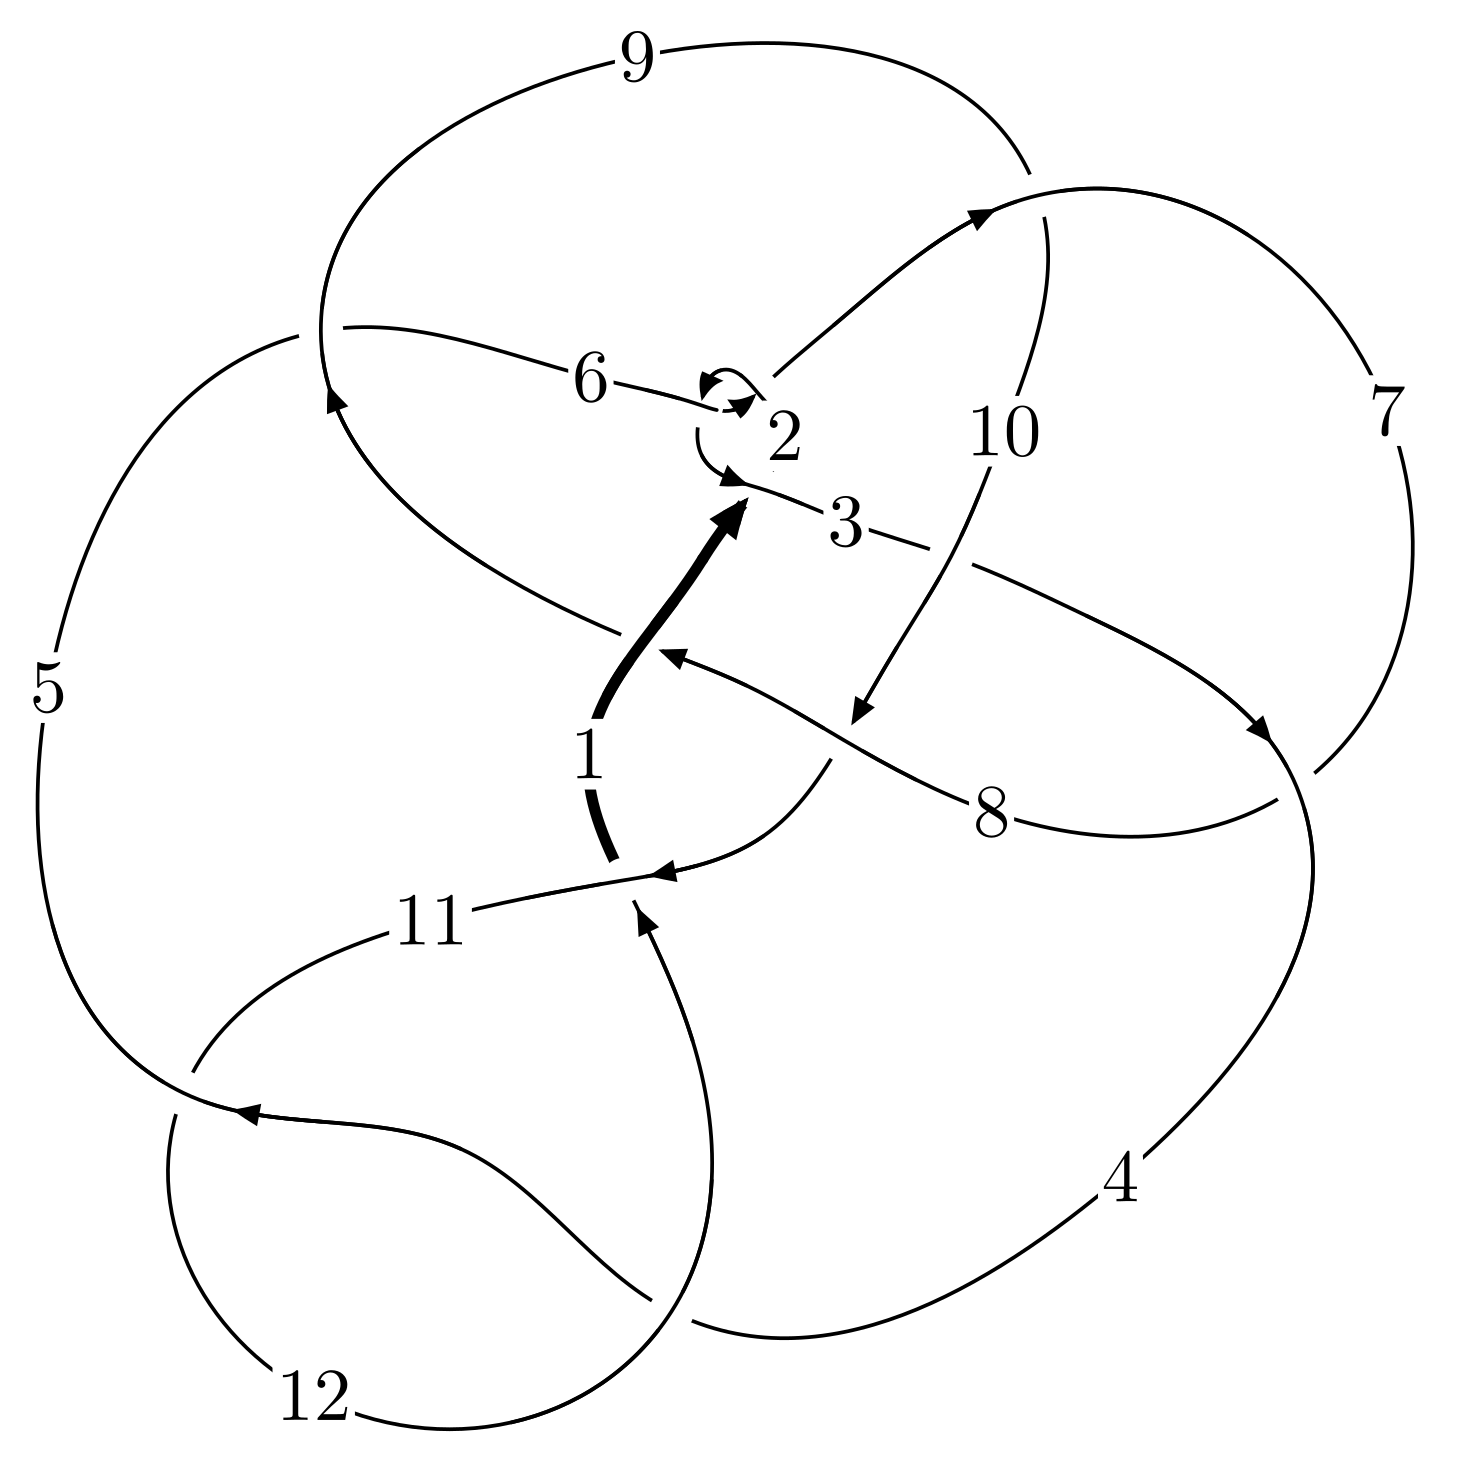
\includegraphics[width=112pt]{../../../GIT/diagram.site/Diagrams/png/1259_12a_0458.png}\\
\ \ \ A knot diagram\footnotemark}&
\allowdisplaybreaks
\textbf{Linearized knot diagam} \\
\cline{2-2}
 &
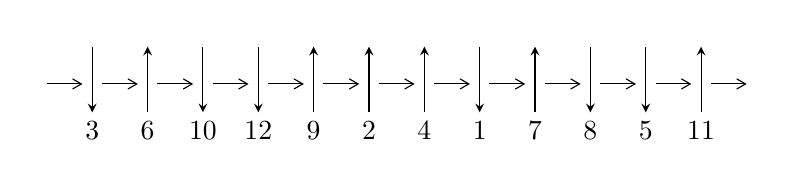
\begin{tikzpicture}[x=20pt, y=17pt]
	% nodes
	\node (C0) at (0, 0) {};
	\node (C1) at (1, 0) {};
	\node (C1U) at (1, +1) {};
	\node (C1D) at (1, -1) {3};

	\node (C2) at (2, 0) {};
	\node (C2U) at (2, +1) {};
	\node (C2D) at (2, -1) {6};

	\node (C3) at (3, 0) {};
	\node (C3U) at (3, +1) {};
	\node (C3D) at (3, -1) {10};

	\node (C4) at (4, 0) {};
	\node (C4U) at (4, +1) {};
	\node (C4D) at (4, -1) {12};

	\node (C5) at (5, 0) {};
	\node (C5U) at (5, +1) {};
	\node (C5D) at (5, -1) {9};

	\node (C6) at (6, 0) {};
	\node (C6U) at (6, +1) {};
	\node (C6D) at (6, -1) {2};

	\node (C7) at (7, 0) {};
	\node (C7U) at (7, +1) {};
	\node (C7D) at (7, -1) {4};

	\node (C8) at (8, 0) {};
	\node (C8U) at (8, +1) {};
	\node (C8D) at (8, -1) {1};

	\node (C9) at (9, 0) {};
	\node (C9U) at (9, +1) {};
	\node (C9D) at (9, -1) {7};

	\node (C10) at (10, 0) {};
	\node (C10U) at (10, +1) {};
	\node (C10D) at (10, -1) {8};

	\node (C11) at (11, 0) {};
	\node (C11U) at (11, +1) {};
	\node (C11D) at (11, -1) {5};

	\node (C12) at (12, 0) {};
	\node (C12U) at (12, +1) {};
	\node (C12D) at (12, -1) {11};
	\node (C13) at (13, 0) {};

	% arrows
	\draw[->,>={angle 60}]
	(C0) edge (C1) (C1) edge (C2) (C2) edge (C3) (C3) edge (C4) (C4) edge (C5) (C5) edge (C6) (C6) edge (C7) (C7) edge (C8) (C8) edge (C9) (C9) edge (C10) (C10) edge (C11) (C11) edge (C12) (C12) edge (C13) ;	\draw[->,>=stealth]
	(C1U) edge (C1D) (C2D) edge (C2U) (C3U) edge (C3D) (C4U) edge (C4D) (C5D) edge (C5U) (C6D) edge (C6U) (C7D) edge (C7U) (C8U) edge (C8D) (C9D) edge (C9U) (C10U) edge (C10D) (C11U) edge (C11D) (C12D) edge (C12U) ;
	\end{tikzpicture} \\
\hhline{~~} \\& 
\textbf{Solving Sequence} \\ \cline{2-2} 
 &
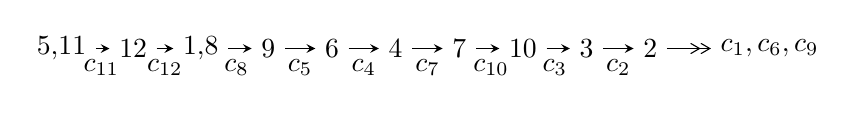
\begin{tikzpicture}[x=23pt, y=7pt]
	% node
	\node (A0) at (-1/8, 0) {5,11};
	\node (A1) at (1, 0) {12};
	\node (A2) at (33/16, 0) {1,8};
	\node (A3) at (25/8, 0) {9};
	\node (A4) at (33/8, 0) {6};
	\node (A5) at (41/8, 0) {4};
	\node (A6) at (49/8, 0) {7};
	\node (A7) at (57/8, 0) {10};
	\node (A8) at (65/8, 0) {3};
	\node (A9) at (73/8, 0) {2};
	\node (C1) at (1/2, -1) {$c_{11}$};
	\node (C2) at (3/2, -1) {$c_{12}$};
	\node (C3) at (21/8, -1) {$c_{8}$};
	\node (C4) at (29/8, -1) {$c_{5}$};
	\node (C5) at (37/8, -1) {$c_{4}$};
	\node (C6) at (45/8, -1) {$c_{7}$};
	\node (C7) at (53/8, -1) {$c_{10}$};
	\node (C8) at (61/8, -1) {$c_{3}$};
	\node (C9) at (69/8, -1) {$c_{2}$};
	\node (A10) at (11, 0) {$c_{1},c_{6},c_{9}$};

	% edge
	\draw[->,>=stealth]	
	(A0) edge (A1) (A1) edge (A2) (A2) edge (A3) (A3) edge (A4) (A4) edge (A5) (A5) edge (A6) (A6) edge (A7) (A7) edge (A8) (A8) edge (A9) ;
	\draw[->>,>={angle 60}]	
	(A9) edge (A10);
\end{tikzpicture} \\ 

\end{tabular} \\

\footnotetext{
The image of knot diagram is generated by the software ``\textbf{Draw programme}" developed by Andrew Bartholomew(\url{http://www.layer8.co.uk/maths/draw/index.htm\#Running-draw}), where we modified some parts for our purpose(\url{https://github.com/CATsTAILs/LinksPainter}).
}\phantom \\ \newline 
\centering \textbf{Ideals for irreducible components\footnotemark of $X_{\text{par}}$} 
 
\begin{align*}
I^u_{1}&=\langle 
-2.50272\times10^{508} u^{183}+4.81379\times10^{508} u^{182}+\cdots+5.05629\times10^{507} b+4.40651\times10^{508},\\
\phantom{I^u_{1}}&\phantom{= \langle  }4.37784\times10^{508} u^{183}-1.28883\times10^{509} u^{182}+\cdots+5.05629\times10^{507} a-1.21040\times10^{509},\;u^{184}- u^{183}+\cdots+5 u+1\rangle \\
I^u_{2}&=\langle 
4318092 u^{35}+4278394 u^{34}+\cdots+627059 b+4485498,\\
\phantom{I^u_{2}}&\phantom{= \langle  }-2296428 u^{35}-6821624 u^{34}+\cdots+627059 a-828341,\;u^{36}+u^{35}+\cdots-2 u+1\rangle \\
I^u_{3}&=\langle 
- u^2+b+u,\;- u^3+u^2+a,\;u^4- u^3+u^2- u+1\rangle \\
\\
\end{align*}
\raggedright * 3 irreducible components of $\dim_{\mathbb{C}}=0$, with total 224 representations.\\
\footnotetext{All coefficients of polynomials are rational numbers. But the coefficients are sometimes approximated in decimal forms when there is not enough margin.}
\newpage
\renewcommand{\arraystretch}{1}
\centering \section*{I. $I^u_{1}= \langle -2.50\times10^{508} u^{183}+4.81\times10^{508} u^{182}+\cdots+5.06\times10^{507} b+4.41\times10^{508},\;4.38\times10^{508} u^{183}-1.29\times10^{509} u^{182}+\cdots+5.06\times10^{507} a-1.21\times10^{509},\;u^{184}- u^{183}+\cdots+5 u+1 \rangle$}
\flushleft \textbf{(i) Arc colorings}\\
\begin{tabular}{m{7pt} m{180pt} m{7pt} m{180pt} }
\flushright $a_{5}=$&$\begin{pmatrix}0\\u\end{pmatrix}$ \\
\flushright $a_{11}=$&$\begin{pmatrix}1\\0\end{pmatrix}$ \\
\flushright $a_{12}=$&$\begin{pmatrix}1\\u^2\end{pmatrix}$ \\
\flushright $a_{1}=$&$\begin{pmatrix}u^2+1\\u^2\end{pmatrix}$ \\
\flushright $a_{8}=$&$\begin{pmatrix}-8.65822 u^{183}+25.4895 u^{182}+\cdots+204.609 u+23.9386\\4.94971 u^{183}-9.52040 u^{182}+\cdots-61.9664 u-8.71491\end{pmatrix}$ \\
\flushright $a_{9}=$&$\begin{pmatrix}0.687710 u^{183}+11.7257 u^{182}+\cdots+124.941 u+5.27965\\-4.07758 u^{183}-10.8828 u^{182}+\cdots-110.199 u-14.6867\end{pmatrix}$ \\
\flushright $a_{6}=$&$\begin{pmatrix}8.59308 u^{183}-23.6383 u^{182}+\cdots-180.726 u-46.3702\\-6.10986 u^{183}-4.33107 u^{182}+\cdots-36.2462 u-4.36522\end{pmatrix}$ \\
\flushright $a_{4}=$&$\begin{pmatrix}u\\u^3+u\end{pmatrix}$ \\
\flushright $a_{7}=$&$\begin{pmatrix}2.90959 u^{183}+7.18098 u^{182}+\cdots+94.9978 u+2.60094\\3.37583 u^{183}-18.8275 u^{182}+\cdots-149.441 u-23.3118\end{pmatrix}$ \\
\flushright $a_{10}=$&$\begin{pmatrix}-10.5685 u^{183}+20.0248 u^{182}+\cdots+118.185 u+26.8545\\23.1516 u^{183}-5.66655 u^{182}+\cdots+10.6861 u-1.74697\end{pmatrix}$ \\
\flushright $a_{3}=$&$\begin{pmatrix}-2.11007 u^{183}+24.7206 u^{182}+\cdots+206.052 u+48.7688\\19.4953 u^{183}+1.85177 u^{182}+\cdots+82.3695 u+7.98087\end{pmatrix}$ \\
\flushright $a_{2}=$&$\begin{pmatrix}17.3504 u^{183}+20.0924 u^{182}+\cdots+166.223 u+39.3952\\40.7180 u^{183}-14.7779 u^{182}+\cdots+14.5445 u-10.5460\end{pmatrix}$\\&\end{tabular}
\flushleft \textbf{(ii) Obstruction class $= -1$}\\~\\
\flushleft \textbf{(iii) Cusp Shapes $= 40.5446 u^{183}-51.3735 u^{182}+\cdots-251.843 u-67.3318$}\\~\\
\newpage\renewcommand{\arraystretch}{1}
\flushleft \textbf{(iv) u-Polynomials at the component}\newline \\
\begin{tabular}{m{50pt}|m{274pt}}
Crossings & \hspace{64pt}u-Polynomials at each crossing \\
\hline $$\begin{aligned}c_{1}\end{aligned}$$&$\begin{aligned}
&u^{184}+83 u^{183}+\cdots-5 u+1
\end{aligned}$\\
\hline $$\begin{aligned}c_{2},c_{6}\end{aligned}$$&$\begin{aligned}
&u^{184}- u^{183}+\cdots+5 u+1
\end{aligned}$\\
\hline $$\begin{aligned}c_{3}\end{aligned}$$&$\begin{aligned}
&u^{184}+2 u^{183}+\cdots+4095 u+691
\end{aligned}$\\
\hline $$\begin{aligned}c_{4},c_{11}\end{aligned}$$&$\begin{aligned}
&u^{184}+u^{183}+\cdots-5 u+1
\end{aligned}$\\
\hline $$\begin{aligned}c_{5}\end{aligned}$$&$\begin{aligned}
&u^{184}+2 u^{183}+\cdots+3708404 u+1584839
\end{aligned}$\\
\hline $$\begin{aligned}c_{7}\end{aligned}$$&$\begin{aligned}
&u^{184}-2 u^{183}+\cdots-4095 u+691
\end{aligned}$\\
\hline $$\begin{aligned}c_{8}\end{aligned}$$&$\begin{aligned}
&u^{184}-2 u^{183}+\cdots-3708404 u+1584839
\end{aligned}$\\
\hline $$\begin{aligned}c_{9}\end{aligned}$$&$\begin{aligned}
&u^{184}-11 u^{183}+\cdots+8744 u+257
\end{aligned}$\\
\hline $$\begin{aligned}c_{10}\end{aligned}$$&$\begin{aligned}
&u^{184}+11 u^{183}+\cdots-8744 u+257
\end{aligned}$\\
\hline $$\begin{aligned}c_{12}\end{aligned}$$&$\begin{aligned}
&u^{184}-83 u^{183}+\cdots+5 u+1
\end{aligned}$\\
\hline
\end{tabular}\\~\\
\newpage\renewcommand{\arraystretch}{1}
\flushleft \textbf{(v) Riley Polynomials at the component}\newline \\
\begin{tabular}{m{50pt}|m{274pt}}
Crossings & \hspace{64pt}Riley Polynomials at each crossing \\
\hline $$\begin{aligned}c_{1},c_{12}\end{aligned}$$&$\begin{aligned}
&y^{184}+47 y^{183}+\cdots-2797 y+1
\end{aligned}$\\
\hline $$\begin{aligned}c_{2},c_{4},c_{6}\\c_{11}\end{aligned}$$&$\begin{aligned}
&y^{184}+83 y^{183}+\cdots-5 y+1
\end{aligned}$\\
\hline $$\begin{aligned}c_{3},c_{7}\end{aligned}$$&$\begin{aligned}
&y^{184}+2 y^{183}+\cdots-20009815 y+477481
\end{aligned}$\\
\hline $$\begin{aligned}c_{5},c_{8}\end{aligned}$$&$\begin{aligned}
&y^{184}-18 y^{183}+\cdots-530431543575720 y+2511714655921
\end{aligned}$\\
\hline $$\begin{aligned}c_{9},c_{10}\end{aligned}$$&$\begin{aligned}
&y^{184}-23 y^{183}+\cdots+38603420 y+66049
\end{aligned}$\\
\hline
\end{tabular}\\~\\
\newpage\flushleft \textbf{(vi) Complex Volumes and Cusp Shapes}
$$\begin{array}{c|c|c}  
\text{Solutions to }I^u_{1}& \I (\text{vol} + \sqrt{-1}CS) & \text{Cusp shape}\\
 \hline 
\begin{aligned}
u &= -0.894854 + 0.445183 I \\
a &= \phantom{-}1.130450 + 0.587646 I \\
b &= \phantom{-}0.870846 + 0.629086 I\end{aligned}
 & \phantom{-}1.42713 - 4.91064 I & \phantom{-0.000000 } 0 \\ \hline\begin{aligned}
u &= -0.894854 - 0.445183 I \\
a &= \phantom{-}1.130450 - 0.587646 I \\
b &= \phantom{-}0.870846 - 0.629086 I\end{aligned}
 & \phantom{-}1.42713 + 4.91064 I & \phantom{-0.000000 } 0 \\ \hline\begin{aligned}
u &= -0.505930 + 0.869761 I \\
a &= -1.11752 - 1.42800 I \\
b &= -0.943800 + 0.915800 I\end{aligned}
 & -2.46244 + 5.69178 I & \phantom{-0.000000 } 0 \\ \hline\begin{aligned}
u &= -0.505930 - 0.869761 I \\
a &= -1.11752 + 1.42800 I \\
b &= -0.943800 - 0.915800 I\end{aligned}
 & -2.46244 - 5.69178 I & \phantom{-0.000000 } 0 \\ \hline\begin{aligned}
u &= \phantom{-}0.711964 + 0.692118 I \\
a &= -0.94076 + 1.54269 I \\
b &= -1.42433 + 0.63907 I\end{aligned}
 & -4.26633 - 0.73149 I & \phantom{-0.000000 } 0 \\ \hline\begin{aligned}
u &= \phantom{-}0.711964 - 0.692118 I \\
a &= -0.94076 - 1.54269 I \\
b &= -1.42433 - 0.63907 I\end{aligned}
 & -4.26633 + 0.73149 I & \phantom{-0.000000 } 0 \\ \hline\begin{aligned}
u &= -0.911661 + 0.428389 I \\
a &= \phantom{-}1.24757 + 0.81419 I \\
b &= \phantom{-}1.21961 + 0.85454 I\end{aligned}
 & \phantom{-0.000000 } -9.45857 I & \phantom{-0.000000 } 0 \\ \hline\begin{aligned}
u &= -0.911661 - 0.428389 I \\
a &= \phantom{-}1.24757 - 0.81419 I \\
b &= \phantom{-}1.21961 - 0.85454 I\end{aligned}
 & \phantom{-0.000000 -}9.45857 I & \phantom{-0.000000 } 0 \\ \hline\begin{aligned}
u &= \phantom{-}0.912513 + 0.427584 I \\
a &= \phantom{-}1.34384 - 0.71854 I \\
b &= \phantom{-}1.259440 - 0.641346 I\end{aligned}
 & -6.16241 + 6.57875 I & \phantom{-0.000000 } 0 \\ \hline\begin{aligned}
u &= \phantom{-}0.912513 - 0.427584 I \\
a &= \phantom{-}1.34384 + 0.71854 I \\
b &= \phantom{-}1.259440 + 0.641346 I\end{aligned}
 & -6.16241 - 6.57875 I & \phantom{-0.000000 } 0\\
 \hline 
 \end{array}$$\newpage$$\begin{array}{c|c|c}  
\text{Solutions to }I^u_{1}& \I (\text{vol} + \sqrt{-1}CS) & \text{Cusp shape}\\
 \hline 
\begin{aligned}
u &= \phantom{-}0.913042 + 0.429711 I \\
a &= \phantom{-}1.27214 - 0.86579 I \\
b &= \phantom{-}1.30328 - 0.90182 I\end{aligned}
 & -2.1765 + 15.2001 I & \phantom{-0.000000 } 0 \\ \hline\begin{aligned}
u &= \phantom{-}0.913042 - 0.429711 I \\
a &= \phantom{-}1.27214 + 0.86579 I \\
b &= \phantom{-}1.30328 + 0.90182 I\end{aligned}
 & -2.1765 - 15.2001 I & \phantom{-0.000000 } 0 \\ \hline\begin{aligned}
u &= -0.480224 + 0.863743 I \\
a &= -0.758550 - 0.515933 I \\
b &= -1.34440 - 0.80705 I\end{aligned}
 & -2.51303 - 1.69167 I & \phantom{-0.000000 } 0 \\ \hline\begin{aligned}
u &= -0.480224 - 0.863743 I \\
a &= -0.758550 + 0.515933 I \\
b &= -1.34440 + 0.80705 I\end{aligned}
 & -2.51303 + 1.69167 I & \phantom{-0.000000 } 0 \\ \hline\begin{aligned}
u &= -0.823126 + 0.594241 I \\
a &= -0.616204 - 1.118430 I \\
b &= -1.10371 - 0.91332 I\end{aligned}
 & -2.93943 - 1.39204 I & \phantom{-0.000000 } 0 \\ \hline\begin{aligned}
u &= -0.823126 - 0.594241 I \\
a &= -0.616204 + 1.118430 I \\
b &= -1.10371 + 0.91332 I\end{aligned}
 & -2.93943 + 1.39204 I & \phantom{-0.000000 } 0 \\ \hline\begin{aligned}
u &= \phantom{-}0.696281 + 0.684139 I \\
a &= \phantom{-}1.50341 + 0.43910 I \\
b &= \phantom{-}0.665119 - 0.261921 I\end{aligned}
 & -0.510482 + 0.490371 I & \phantom{-0.000000 } 0 \\ \hline\begin{aligned}
u &= \phantom{-}0.696281 - 0.684139 I \\
a &= \phantom{-}1.50341 - 0.43910 I \\
b &= \phantom{-}0.665119 + 0.261921 I\end{aligned}
 & -0.510482 - 0.490371 I & \phantom{-0.000000 } 0 \\ \hline\begin{aligned}
u &= \phantom{-}0.152840 + 0.963831 I \\
a &= \phantom{-}1.166230 - 0.182836 I \\
b &= -0.463762 + 0.579118 I\end{aligned}
 & -0.16328 - 1.51231 I & \phantom{-0.000000 } 0 \\ \hline\begin{aligned}
u &= \phantom{-}0.152840 - 0.963831 I \\
a &= \phantom{-}1.166230 + 0.182836 I \\
b &= -0.463762 - 0.579118 I\end{aligned}
 & -0.16328 + 1.51231 I & \phantom{-0.000000 } 0\\
 \hline 
 \end{array}$$\newpage$$\begin{array}{c|c|c}  
\text{Solutions to }I^u_{1}& \I (\text{vol} + \sqrt{-1}CS) & \text{Cusp shape}\\
 \hline 
\begin{aligned}
u &= \phantom{-}0.381338 + 0.953885 I \\
a &= \phantom{-}1.53715 - 0.34005 I \\
b &= \phantom{-}0.504853 + 0.770017 I\end{aligned}
 & \phantom{-}0.16328 - 1.51231 I & \phantom{-0.000000 } 0 \\ \hline\begin{aligned}
u &= \phantom{-}0.381338 - 0.953885 I \\
a &= \phantom{-}1.53715 + 0.34005 I \\
b &= \phantom{-}0.504853 - 0.770017 I\end{aligned}
 & \phantom{-}0.16328 + 1.51231 I & \phantom{-0.000000 } 0 \\ \hline\begin{aligned}
u &= \phantom{-}0.843737 + 0.481906 I \\
a &= \phantom{-}1.036830 - 0.436222 I \\
b &= \phantom{-}0.636621 - 0.450084 I\end{aligned}
 & \phantom{-}0.606146 - 1.140740 I & \phantom{-0.000000 } 0 \\ \hline\begin{aligned}
u &= \phantom{-}0.843737 - 0.481906 I \\
a &= \phantom{-}1.036830 + 0.436222 I \\
b &= \phantom{-}0.636621 + 0.450084 I\end{aligned}
 & \phantom{-}0.606146 + 1.140740 I & \phantom{-0.000000 } 0 \\ \hline\begin{aligned}
u &= \phantom{-}0.793686 + 0.656060 I \\
a &= -0.67850 + 1.38327 I \\
b &= -1.32553 + 0.93427 I\end{aligned}
 & -3.89040 + 5.00488 I & \phantom{-0.000000 } 0 \\ \hline\begin{aligned}
u &= \phantom{-}0.793686 - 0.656060 I \\
a &= -0.67850 - 1.38327 I \\
b &= -1.32553 - 0.93427 I\end{aligned}
 & -3.89040 - 5.00488 I & \phantom{-0.000000 } 0 \\ \hline\begin{aligned}
u &= \phantom{-}0.487021 + 0.908990 I \\
a &= -1.382000 - 0.167841 I \\
b &= -0.933256 + 0.346925 I\end{aligned}
 & \phantom{-}0.67186 - 2.31975 I & \phantom{-0.000000 } 0 \\ \hline\begin{aligned}
u &= \phantom{-}0.487021 - 0.908990 I \\
a &= -1.382000 + 0.167841 I \\
b &= -0.933256 - 0.346925 I\end{aligned}
 & \phantom{-}0.67186 + 2.31975 I & \phantom{-0.000000 } 0 \\ \hline\begin{aligned}
u &= -0.258634 + 1.001010 I \\
a &= \phantom{-}1.026540 + 0.626638 I \\
b &= -0.608734 - 1.144460 I\end{aligned}
 & \phantom{-}1.179990 - 0.430240 I & \phantom{-0.000000 } 0 \\ \hline\begin{aligned}
u &= -0.258634 - 1.001010 I \\
a &= \phantom{-}1.026540 - 0.626638 I \\
b &= -0.608734 + 1.144460 I\end{aligned}
 & \phantom{-}1.179990 + 0.430240 I & \phantom{-0.000000 } 0\\
 \hline 
 \end{array}$$\newpage$$\begin{array}{c|c|c}  
\text{Solutions to }I^u_{1}& \I (\text{vol} + \sqrt{-1}CS) & \text{Cusp shape}\\
 \hline 
\begin{aligned}
u &= \phantom{-}0.377689 + 0.965511 I \\
a &= \phantom{-}2.36112 - 0.96293 I \\
b &= \phantom{-}1.33765 + 1.31026 I\end{aligned}
 & \phantom{-}2.95745 + 5.07220 I & \phantom{-0.000000 } 0 \\ \hline\begin{aligned}
u &= \phantom{-}0.377689 - 0.965511 I \\
a &= \phantom{-}2.36112 + 0.96293 I \\
b &= \phantom{-}1.33765 - 1.31026 I\end{aligned}
 & \phantom{-}2.95745 - 5.07220 I & \phantom{-0.000000 } 0 \\ \hline\begin{aligned}
u &= \phantom{-}0.200530 + 1.018050 I \\
a &= \phantom{-}1.186000 - 0.505365 I \\
b &= -0.710658 + 0.984129 I\end{aligned}
 & \phantom{-}0.36441 + 4.08864 I & \phantom{-0.000000 } 0 \\ \hline\begin{aligned}
u &= \phantom{-}0.200530 - 1.018050 I \\
a &= \phantom{-}1.186000 + 0.505365 I \\
b &= -0.710658 - 0.984129 I\end{aligned}
 & \phantom{-}0.36441 - 4.08864 I & \phantom{-0.000000 } 0 \\ \hline\begin{aligned}
u &= -0.373627 + 0.969972 I \\
a &= \phantom{-}2.00297 + 1.12039 I \\
b &= \phantom{-}1.36042 - 0.96472 I\end{aligned}
 & \phantom{-}4.76977 - 0.02280 I & \phantom{-0.000000 } 0 \\ \hline\begin{aligned}
u &= -0.373627 - 0.969972 I \\
a &= \phantom{-}2.00297 - 1.12039 I \\
b &= \phantom{-}1.36042 + 0.96472 I\end{aligned}
 & \phantom{-}4.76977 + 0.02280 I & \phantom{-0.000000 } 0 \\ \hline\begin{aligned}
u &= -0.536403 + 0.906961 I \\
a &= -1.74681 - 0.53934 I \\
b &= -1.42395 + 0.11348 I\end{aligned}
 & -2.99007 + 5.88748 I & \phantom{-0.000000 } 0 \\ \hline\begin{aligned}
u &= -0.536403 - 0.906961 I \\
a &= -1.74681 + 0.53934 I \\
b &= -1.42395 - 0.11348 I\end{aligned}
 & -2.99007 - 5.88748 I & \phantom{-0.000000 } 0 \\ \hline\begin{aligned}
u &= -0.713873 + 0.612272 I \\
a &= \phantom{-}1.213510 - 0.492034 I \\
b &= \phantom{-}0.798352 + 0.374709 I\end{aligned}
 & -2.75046 - 6.50723 I & \phantom{-0.000000 } 0 \\ \hline\begin{aligned}
u &= -0.713873 - 0.612272 I \\
a &= \phantom{-}1.213510 + 0.492034 I \\
b &= \phantom{-}0.798352 - 0.374709 I\end{aligned}
 & -2.75046 + 6.50723 I & \phantom{-0.000000 } 0\\
 \hline 
 \end{array}$$\newpage$$\begin{array}{c|c|c}  
\text{Solutions to }I^u_{1}& \I (\text{vol} + \sqrt{-1}CS) & \text{Cusp shape}\\
 \hline 
\begin{aligned}
u &= \phantom{-}0.463990 + 0.816495 I \\
a &= -0.73359 + 1.81235 I \\
b &= -0.541609 - 0.530760 I\end{aligned}
 & \phantom{-}0.33646 - 1.58880 I & \phantom{-0.000000 } 0 \\ \hline\begin{aligned}
u &= \phantom{-}0.463990 - 0.816495 I \\
a &= -0.73359 - 1.81235 I \\
b &= -0.541609 + 0.530760 I\end{aligned}
 & \phantom{-}0.33646 + 1.58880 I & \phantom{-0.000000 } 0 \\ \hline\begin{aligned}
u &= -0.549717 + 0.760668 I \\
a &= -1.20472 - 1.75793 I \\
b &= -1.051140 + 0.039586 I\end{aligned}
 & -3.43015 - 1.51038 I & \phantom{-0.000000 } 0 \\ \hline\begin{aligned}
u &= -0.549717 - 0.760668 I \\
a &= -1.20472 + 1.75793 I \\
b &= -1.051140 - 0.039586 I\end{aligned}
 & -3.43015 + 1.51038 I & \phantom{-0.000000 } 0 \\ \hline\begin{aligned}
u &= -0.840506 + 0.652157 I \\
a &= \phantom{-}1.053580 - 0.135131 I \\
b &= \phantom{-}0.905372 + 0.023325 I\end{aligned}
 & -7.61513 + 2.24725 I & \phantom{-0.000000 } 0 \\ \hline\begin{aligned}
u &= -0.840506 - 0.652157 I \\
a &= \phantom{-}1.053580 + 0.135131 I \\
b &= \phantom{-}0.905372 - 0.023325 I\end{aligned}
 & -7.61513 - 2.24725 I & \phantom{-0.000000 } 0 \\ \hline\begin{aligned}
u &= -0.356964 + 1.003780 I \\
a &= \phantom{-}1.10995 + 1.34623 I \\
b &= \phantom{-}1.363320 - 0.196047 I\end{aligned}
 & \phantom{-}4.71361 + 2.34843 I & \phantom{-0.000000 } 0 \\ \hline\begin{aligned}
u &= -0.356964 - 1.003780 I \\
a &= \phantom{-}1.10995 - 1.34623 I \\
b &= \phantom{-}1.363320 + 0.196047 I\end{aligned}
 & \phantom{-}4.71361 - 2.34843 I & \phantom{-0.000000 } 0 \\ \hline\begin{aligned}
u &= \phantom{-}0.414228 + 0.981909 I \\
a &= \phantom{-}0.354458 - 1.062160 I \\
b &= -0.371091 + 1.052520 I\end{aligned}
 & \phantom{-}4.26633 - 0.73149 I & \phantom{-0.000000 } 0 \\ \hline\begin{aligned}
u &= \phantom{-}0.414228 - 0.981909 I \\
a &= \phantom{-}0.354458 + 1.062160 I \\
b &= -0.371091 - 1.052520 I\end{aligned}
 & \phantom{-}4.26633 + 0.73149 I & \phantom{-0.000000 } 0\\
 \hline 
 \end{array}$$\newpage$$\begin{array}{c|c|c}  
\text{Solutions to }I^u_{1}& \I (\text{vol} + \sqrt{-1}CS) & \text{Cusp shape}\\
 \hline 
\begin{aligned}
u &= -0.129488 + 0.915164 I \\
a &= \phantom{-}0.960675 + 0.426662 I \\
b &= -0.296636 - 0.987355 I\end{aligned}
 & \phantom{-}1.82416 - 1.29895 I & \phantom{-0.000000 } 0 \\ \hline\begin{aligned}
u &= -0.129488 - 0.915164 I \\
a &= \phantom{-}0.960675 - 0.426662 I \\
b &= -0.296636 + 0.987355 I\end{aligned}
 & \phantom{-}1.82416 + 1.29895 I & \phantom{-0.000000 } 0 \\ \hline\begin{aligned}
u &= -0.383178 + 1.005400 I \\
a &= \phantom{-}0.618638 + 1.012630 I \\
b &= -0.393790 - 1.184510 I\end{aligned}
 & \phantom{-}3.42616 - 4.42719 I & \phantom{-0.000000 } 0 \\ \hline\begin{aligned}
u &= -0.383178 - 1.005400 I \\
a &= \phantom{-}0.618638 - 1.012630 I \\
b &= -0.393790 + 1.184510 I\end{aligned}
 & \phantom{-}3.42616 + 4.42719 I & \phantom{-0.000000 } 0 \\ \hline\begin{aligned}
u &= \phantom{-}0.321449 + 1.031970 I \\
a &= \phantom{-}0.62025 - 1.47461 I \\
b &= \phantom{-}1.41421 - 0.14004 I\end{aligned}
 & \phantom{-}2.71913 - 7.28797 I & \phantom{-0.000000 } 0 \\ \hline\begin{aligned}
u &= \phantom{-}0.321449 - 1.031970 I \\
a &= \phantom{-}0.62025 + 1.47461 I \\
b &= \phantom{-}1.41421 + 0.14004 I\end{aligned}
 & \phantom{-}2.71913 + 7.28797 I & \phantom{-0.000000 } 0 \\ \hline\begin{aligned}
u &= \phantom{-}0.481357 + 0.968112 I \\
a &= -1.053720 - 0.021626 I \\
b &= \phantom{-}0.07893 - 1.73838 I\end{aligned}
 & -0.36441 - 4.08864 I & \phantom{-0.000000 } 0 \\ \hline\begin{aligned}
u &= \phantom{-}0.481357 - 0.968112 I \\
a &= -1.053720 + 0.021626 I \\
b &= \phantom{-}0.07893 + 1.73838 I\end{aligned}
 & -0.36441 + 4.08864 I & \phantom{-0.000000 } 0 \\ \hline\begin{aligned}
u &= \phantom{-}0.477961 + 0.978704 I \\
a &= -2.55928 + 0.63156 I \\
b &= -0.540892 - 0.552874 I\end{aligned}
 & \phantom{-}3.89040 - 5.00488 I & \phantom{-0.000000 } 0 \\ \hline\begin{aligned}
u &= \phantom{-}0.477961 - 0.978704 I \\
a &= -2.55928 - 0.63156 I \\
b &= -0.540892 + 0.552874 I\end{aligned}
 & \phantom{-}3.89040 + 5.00488 I & \phantom{-0.000000 } 0\\
 \hline 
 \end{array}$$\newpage$$\begin{array}{c|c|c}  
\text{Solutions to }I^u_{1}& \I (\text{vol} + \sqrt{-1}CS) & \text{Cusp shape}\\
 \hline 
\begin{aligned}
u &= \phantom{-}0.288183 + 1.051500 I \\
a &= \phantom{-}0.451947 + 0.568551 I \\
b &= -0.168159 - 0.824343 I\end{aligned}
 & \phantom{-}3.43015 - 1.51038 I & \phantom{-0.000000 } 0 \\ \hline\begin{aligned}
u &= \phantom{-}0.288183 - 1.051500 I \\
a &= \phantom{-}0.451947 - 0.568551 I \\
b &= -0.168159 + 0.824343 I\end{aligned}
 & \phantom{-}3.43015 + 1.51038 I & \phantom{-0.000000 } 0 \\ \hline\begin{aligned}
u &= \phantom{-}0.997685 + 0.442110 I \\
a &= -0.260668 + 0.432401 I \\
b &= -0.503103 + 0.532034 I\end{aligned}
 & \phantom{-}0.510482 + 0.490371 I & \phantom{-0.000000 } 0 \\ \hline\begin{aligned}
u &= \phantom{-}0.997685 - 0.442110 I \\
a &= -0.260668 - 0.432401 I \\
b &= -0.503103 - 0.532034 I\end{aligned}
 & \phantom{-}0.510482 - 0.490371 I & \phantom{-0.000000 } 0 \\ \hline\begin{aligned}
u &= -0.965634 + 0.515995 I \\
a &= -0.226054 - 0.635251 I \\
b &= -0.543836 - 0.760332 I\end{aligned}
 & -0.39103 - 5.61584 I & \phantom{-0.000000 } 0 \\ \hline\begin{aligned}
u &= -0.965634 - 0.515995 I \\
a &= -0.226054 + 0.635251 I \\
b &= -0.543836 + 0.760332 I\end{aligned}
 & -0.39103 + 5.61584 I & \phantom{-0.000000 } 0 \\ \hline\begin{aligned}
u &= -0.899610 + 0.655284 I \\
a &= \phantom{-}0.891423 - 0.168943 I \\
b &= \phantom{-}0.942689 - 0.215527 I\end{aligned}
 & -3.50746 + 10.61500 I & \phantom{-0.000000 } 0 \\ \hline\begin{aligned}
u &= -0.899610 - 0.655284 I \\
a &= \phantom{-}0.891423 + 0.168943 I \\
b &= \phantom{-}0.942689 + 0.215527 I\end{aligned}
 & -3.50746 - 10.61500 I & \phantom{-0.000000 } 0 \\ \hline\begin{aligned}
u &= \phantom{-}0.508993 + 0.990974 I \\
a &= -1.19790 - 0.86056 I \\
b &= \phantom{-}0.77945 - 2.15645 I\end{aligned}
 & \phantom{-}2.08454 - 10.78560 I & \phantom{-0.000000 } 0 \\ \hline\begin{aligned}
u &= \phantom{-}0.508993 - 0.990974 I \\
a &= -1.19790 + 0.86056 I \\
b &= \phantom{-}0.77945 + 2.15645 I\end{aligned}
 & \phantom{-}2.08454 + 10.78560 I & \phantom{-0.000000 } 0\\
 \hline 
 \end{array}$$\newpage$$\begin{array}{c|c|c}  
\text{Solutions to }I^u_{1}& \I (\text{vol} + \sqrt{-1}CS) & \text{Cusp shape}\\
 \hline 
\begin{aligned}
u &= -0.483626 + 1.004630 I \\
a &= -2.46022 - 0.80412 I \\
b &= -0.550966 + 0.771385 I\end{aligned}
 & \phantom{-}2.80619 + 10.52050 I & \phantom{-0.000000 } 0 \\ \hline\begin{aligned}
u &= -0.483626 - 1.004630 I \\
a &= -2.46022 + 0.80412 I \\
b &= -0.550966 - 0.771385 I\end{aligned}
 & \phantom{-}2.80619 - 10.52050 I & \phantom{-0.000000 } 0 \\ \hline\begin{aligned}
u &= \phantom{-}0.887503 + 0.675169 I \\
a &= \phantom{-}0.889093 + 0.104858 I \\
b &= \phantom{-}0.856581 + 0.175152 I\end{aligned}
 & -1.42713 - 4.91064 I & \phantom{-0.000000 } 0 \\ \hline\begin{aligned}
u &= \phantom{-}0.887503 - 0.675169 I \\
a &= \phantom{-}0.889093 - 0.104858 I \\
b &= \phantom{-}0.856581 - 0.175152 I\end{aligned}
 & -1.42713 + 4.91064 I & \phantom{-0.000000 } 0 \\ \hline\begin{aligned}
u &= -0.686763 + 0.553968 I \\
a &= -1.15225 - 1.14999 I \\
b &= -1.155710 - 0.749097 I\end{aligned}
 & -2.63356 - 2.12680 I & \phantom{-0.000000 } 0 \\ \hline\begin{aligned}
u &= -0.686763 - 0.553968 I \\
a &= -1.15225 + 1.14999 I \\
b &= -1.155710 + 0.749097 I\end{aligned}
 & -2.63356 + 2.12680 I & \phantom{-0.000000 } 0 \\ \hline\begin{aligned}
u &= -0.499533 + 1.001820 I \\
a &= -0.859826 + 0.800973 I \\
b &= \phantom{-}0.83318 + 1.81298 I\end{aligned}
 & \phantom{-}3.92280 + 5.88359 I & \phantom{-0.000000 } 0 \\ \hline\begin{aligned}
u &= -0.499533 - 1.001820 I \\
a &= -0.859826 - 0.800973 I \\
b &= \phantom{-}0.83318 - 1.81298 I\end{aligned}
 & \phantom{-}3.92280 - 5.88359 I & \phantom{-0.000000 } 0 \\ \hline\begin{aligned}
u &= \phantom{-}0.381904 + 0.774779 I \\
a &= \phantom{-}0.963184 + 0.422425 I \\
b &= -0.59196 + 1.67135 I\end{aligned}
 & -1.179990 + 0.430240 I & \phantom{-0.000000 } 0 \\ \hline\begin{aligned}
u &= \phantom{-}0.381904 - 0.774779 I \\
a &= \phantom{-}0.963184 - 0.422425 I \\
b &= -0.59196 - 1.67135 I\end{aligned}
 & -1.179990 - 0.430240 I & \phantom{-0.000000 } 0\\
 \hline 
 \end{array}$$\newpage$$\begin{array}{c|c|c}  
\text{Solutions to }I^u_{1}& \I (\text{vol} + \sqrt{-1}CS) & \text{Cusp shape}\\
 \hline 
\begin{aligned}
u &= \phantom{-}0.727245 + 0.460284 I \\
a &= -1.33174 + 0.72097 I \\
b &= -1.47714 + 0.71726 I\end{aligned}
 & -4.76977 + 0.02280 I & \phantom{-0.000000 } 0 \\ \hline\begin{aligned}
u &= \phantom{-}0.727245 - 0.460284 I \\
a &= -1.33174 - 0.72097 I \\
b &= -1.47714 - 0.71726 I\end{aligned}
 & -4.76977 - 0.02280 I & \phantom{-0.000000 } 0 \\ \hline\begin{aligned}
u &= -0.471708 + 1.045510 I \\
a &= -0.057598 + 0.754177 I \\
b &= \phantom{-}0.962909 + 0.998986 I\end{aligned}
 & \phantom{-}3.94857 + 4.14341 I & \phantom{-0.000000 } 0 \\ \hline\begin{aligned}
u &= -0.471708 - 1.045510 I \\
a &= -0.057598 - 0.754177 I \\
b &= \phantom{-}0.962909 - 0.998986 I\end{aligned}
 & \phantom{-}3.94857 - 4.14341 I & \phantom{-0.000000 } 0 \\ \hline\begin{aligned}
u &= -0.337591 + 1.098550 I \\
a &= \phantom{-}0.591677 - 0.468827 I \\
b &= -0.236721 + 0.673392 I\end{aligned}
 & \phantom{-}2.99007 + 5.88748 I & \phantom{-0.000000 } 0 \\ \hline\begin{aligned}
u &= -0.337591 - 1.098550 I \\
a &= \phantom{-}0.591677 + 0.468827 I \\
b &= -0.236721 - 0.673392 I\end{aligned}
 & \phantom{-}2.99007 - 5.88748 I & \phantom{-0.000000 } 0 \\ \hline\begin{aligned}
u &= \phantom{-}0.631075 + 0.965174 I \\
a &= -1.92745 + 0.64474 I \\
b &= -1.55707 - 1.01380 I\end{aligned}
 & -3.42616 - 4.42719 I & \phantom{-0.000000 } 0 \\ \hline\begin{aligned}
u &= \phantom{-}0.631075 - 0.965174 I \\
a &= -1.92745 - 0.64474 I \\
b &= -1.55707 + 1.01380 I\end{aligned}
 & -3.42616 + 4.42719 I & \phantom{-0.000000 } 0 \\ \hline\begin{aligned}
u &= \phantom{-}0.629650 + 0.976191 I \\
a &= \phantom{-}1.23250 - 1.48669 I \\
b &= \phantom{-}0.528126 + 0.382461 I\end{aligned}
 & \phantom{-}0.39103 - 5.61584 I & \phantom{-0.000000 } 0 \\ \hline\begin{aligned}
u &= \phantom{-}0.629650 - 0.976191 I \\
a &= \phantom{-}1.23250 + 1.48669 I \\
b &= \phantom{-}0.528126 - 0.382461 I\end{aligned}
 & \phantom{-}0.39103 + 5.61584 I & \phantom{-0.000000 } 0\\
 \hline 
 \end{array}$$\newpage$$\begin{array}{c|c|c}  
\text{Solutions to }I^u_{1}& \I (\text{vol} + \sqrt{-1}CS) & \text{Cusp shape}\\
 \hline 
\begin{aligned}
u &= \phantom{-}0.352055 + 0.754820 I \\
a &= -2.00994 + 2.12921 I \\
b &= -0.146379 + 0.209850 I\end{aligned}
 & \phantom{-}2.93943 + 1.39204 I & \phantom{-0.000000 } 0 \\ \hline\begin{aligned}
u &= \phantom{-}0.352055 - 0.754820 I \\
a &= -2.00994 - 2.12921 I \\
b &= -0.146379 - 0.209850 I\end{aligned}
 & \phantom{-}2.93943 - 1.39204 I & \phantom{-0.000000 } 0 \\ \hline\begin{aligned}
u &= -0.708371 + 0.431036 I \\
a &= -1.293870 - 0.230762 I \\
b &= -1.41656 - 0.14464 I\end{aligned}
 & -4.71361 - 2.34843 I & \phantom{-0.000000 } 0 \\ \hline\begin{aligned}
u &= -0.708371 - 0.431036 I \\
a &= -1.293870 + 0.230762 I \\
b &= -1.41656 + 0.14464 I\end{aligned}
 & -4.71361 + 2.34843 I & \phantom{-0.000000 } 0 \\ \hline\begin{aligned}
u &= \phantom{-}0.455227 + 1.089340 I \\
a &= \phantom{-}0.974536 - 0.050067 I \\
b &= \phantom{-}0.0693944 - 0.0112381 I\end{aligned}
 & \phantom{-}2.46244 - 5.69178 I & \phantom{-0.000000 } 0 \\ \hline\begin{aligned}
u &= \phantom{-}0.455227 - 1.089340 I \\
a &= \phantom{-}0.974536 + 0.050067 I \\
b &= \phantom{-}0.0693944 + 0.0112381 I\end{aligned}
 & \phantom{-}2.46244 + 5.69178 I & \phantom{-0.000000 } 0 \\ \hline\begin{aligned}
u &= \phantom{-}0.688567 + 0.441057 I \\
a &= -1.40211 + 0.89740 I \\
b &= -1.30493 + 1.02462 I\end{aligned}
 & -3.92280 + 5.88359 I & \phantom{-0.000000 } 0 \\ \hline\begin{aligned}
u &= \phantom{-}0.688567 - 0.441057 I \\
a &= -1.40211 - 0.89740 I \\
b &= -1.30493 - 1.02462 I\end{aligned}
 & -3.92280 - 5.88359 I & \phantom{-0.000000 } 0 \\ \hline\begin{aligned}
u &= -0.419510 + 1.107550 I \\
a &= \phantom{-}0.856484 - 0.171836 I \\
b &= -0.130336 + 0.242419 I\end{aligned}
 & \phantom{-}2.51303 + 1.69167 I & \phantom{-0.000000 } 0 \\ \hline\begin{aligned}
u &= -0.419510 - 1.107550 I \\
a &= \phantom{-}0.856484 + 0.171836 I \\
b &= -0.130336 - 0.242419 I\end{aligned}
 & \phantom{-}2.51303 - 1.69167 I & \phantom{-0.000000 } 0\\
 \hline 
 \end{array}$$\newpage$$\begin{array}{c|c|c}  
\text{Solutions to }I^u_{1}& \I (\text{vol} + \sqrt{-1}CS) & \text{Cusp shape}\\
 \hline 
\begin{aligned}
u &= -0.626190 + 1.006950 I \\
a &= \phantom{-}0.98225 + 1.52642 I \\
b &= \phantom{-}0.596201 - 0.476832 I\end{aligned}
 & -1.56303 + 11.65710 I & \phantom{-0.000000 } 0 \\ \hline\begin{aligned}
u &= -0.626190 - 1.006950 I \\
a &= \phantom{-}0.98225 - 1.52642 I \\
b &= \phantom{-}0.596201 + 0.476832 I\end{aligned}
 & -1.56303 - 11.65710 I & \phantom{-0.000000 } 0 \\ \hline\begin{aligned}
u &= -0.639333 + 0.496386 I \\
a &= -1.37503 - 1.08086 I \\
b &= -1.082360 - 0.869374 I\end{aligned}
 & -2.56168 - 2.03706 I & \phantom{-0.000000 } 0 \\ \hline\begin{aligned}
u &= -0.639333 - 0.496386 I \\
a &= -1.37503 + 1.08086 I \\
b &= -1.082360 + 0.869374 I\end{aligned}
 & -2.56168 + 2.03706 I & \phantom{-0.000000 } 0 \\ \hline\begin{aligned}
u &= \phantom{-}0.381601 + 0.713137 I \\
a &= \phantom{-}1.096170 - 0.184203 I \\
b &= \phantom{-}0.159797 + 0.195526 I\end{aligned}
 & \phantom{-0.000000 } -1.68467 I & \phantom{-0.000000 } 0 \\ \hline\begin{aligned}
u &= \phantom{-}0.381601 - 0.713137 I \\
a &= \phantom{-}1.096170 + 0.184203 I \\
b &= \phantom{-}0.159797 - 0.195526 I\end{aligned}
 & \phantom{-0.000000 -}1.68467 I & \phantom{-0.000000 } 0 \\ \hline\begin{aligned}
u &= -0.571186 + 1.051590 I \\
a &= -1.93792 - 1.06331 I \\
b &= -1.16702 + 1.19477 I\end{aligned}
 & -0.91389 + 6.81255 I & \phantom{-0.000000 } 0 \\ \hline\begin{aligned}
u &= -0.571186 - 1.051590 I \\
a &= -1.93792 + 1.06331 I \\
b &= -1.16702 - 1.19477 I\end{aligned}
 & -0.91389 - 6.81255 I & \phantom{-0.000000 } 0 \\ \hline\begin{aligned}
u &= -0.611075 + 1.029990 I \\
a &= -1.77487 - 0.80064 I \\
b &= -1.27397 + 1.09185 I\end{aligned}
 & -1.22565 + 7.16377 I & \phantom{-0.000000 } 0 \\ \hline\begin{aligned}
u &= -0.611075 - 1.029990 I \\
a &= -1.77487 + 0.80064 I \\
b &= -1.27397 - 1.09185 I\end{aligned}
 & -1.22565 - 7.16377 I & \phantom{-0.000000 } 0\\
 \hline 
 \end{array}$$\newpage$$\begin{array}{c|c|c}  
\text{Solutions to }I^u_{1}& \I (\text{vol} + \sqrt{-1}CS) & \text{Cusp shape}\\
 \hline 
\begin{aligned}
u &= \phantom{-}0.466709 + 1.107420 I \\
a &= \phantom{-}0.335162 - 0.964918 I \\
b &= \phantom{-}1.262510 - 0.540668 I\end{aligned}
 & \phantom{-}1.71729 + 0.12884 I & \phantom{-0.000000 } 0 \\ \hline\begin{aligned}
u &= \phantom{-}0.466709 - 1.107420 I \\
a &= \phantom{-}0.335162 + 0.964918 I \\
b &= \phantom{-}1.262510 + 0.540668 I\end{aligned}
 & \phantom{-}1.71729 - 0.12884 I & \phantom{-0.000000 } 0 \\ \hline\begin{aligned}
u &= \phantom{-}0.671010 + 1.006380 I \\
a &= -1.81191 + 0.52143 I \\
b &= -1.41030 - 1.30320 I\end{aligned}
 & -2.80619 - 10.52050 I & \phantom{-0.000000 } 0 \\ \hline\begin{aligned}
u &= \phantom{-}0.671010 - 1.006380 I \\
a &= -1.81191 - 0.52143 I \\
b &= -1.41030 + 1.30320 I\end{aligned}
 & -2.80619 + 10.52050 I & \phantom{-0.000000 } 0 \\ \hline\begin{aligned}
u &= \phantom{-}0.771291 + 0.937193 I \\
a &= \phantom{-}0.686302 - 0.575965 I \\
b &= \phantom{-}0.616297 + 0.140686 I\end{aligned}
 & -0.606146 - 1.140740 I & \phantom{-0.000000 } 0 \\ \hline\begin{aligned}
u &= \phantom{-}0.771291 - 0.937193 I \\
a &= \phantom{-}0.686302 + 0.575965 I \\
b &= \phantom{-}0.616297 - 0.140686 I\end{aligned}
 & -0.606146 + 1.140740 I & \phantom{-0.000000 } 0 \\ \hline\begin{aligned}
u &= -0.698063 + 0.995619 I \\
a &= \phantom{-}0.841382 + 1.013130 I \\
b &= \phantom{-}0.695453 - 0.262974 I\end{aligned}
 & -6.56925 + 3.46231 I & \phantom{-0.000000 } 0 \\ \hline\begin{aligned}
u &= -0.698063 - 0.995619 I \\
a &= \phantom{-}0.841382 - 1.013130 I \\
b &= \phantom{-}0.695453 + 0.262974 I\end{aligned}
 & -6.56925 - 3.46231 I & \phantom{-0.000000 } 0 \\ \hline\begin{aligned}
u &= \phantom{-}0.578191 + 1.071130 I \\
a &= -1.86866 + 1.25531 I \\
b &= -1.30169 - 1.31275 I\end{aligned}
 & -2.08454 - 10.78560 I & \phantom{-0.000000 } 0 \\ \hline\begin{aligned}
u &= \phantom{-}0.578191 - 1.071130 I \\
a &= -1.86866 - 1.25531 I \\
b &= -1.30169 + 1.31275 I\end{aligned}
 & -2.08454 + 10.78560 I & \phantom{-0.000000 } 0\\
 \hline 
 \end{array}$$\newpage$$\begin{array}{c|c|c}  
\text{Solutions to }I^u_{1}& \I (\text{vol} + \sqrt{-1}CS) & \text{Cusp shape}\\
 \hline 
\begin{aligned}
u &= \phantom{-}0.592842 + 1.073840 I \\
a &= -1.54460 + 1.30495 I \\
b &= -1.47667 - 1.10479 I\end{aligned}
 & -2.95745 - 5.07220 I & \phantom{-0.000000 } 0 \\ \hline\begin{aligned}
u &= \phantom{-}0.592842 - 1.073840 I \\
a &= -1.54460 - 1.30495 I \\
b &= -1.47667 + 1.10479 I\end{aligned}
 & -2.95745 + 5.07220 I & \phantom{-0.000000 } 0 \\ \hline\begin{aligned}
u &= -0.765303 + 0.050024 I \\
a &= \phantom{-}0.363568 + 0.066459 I \\
b &= -0.605791 + 0.141338 I\end{aligned}
 & -0.67186 + 2.31975 I & \phantom{-0.000000 } 0 \\ \hline\begin{aligned}
u &= -0.765303 - 0.050024 I \\
a &= \phantom{-}0.363568 - 0.066459 I \\
b &= -0.605791 - 0.141338 I\end{aligned}
 & -0.67186 - 2.31975 I & \phantom{-0.000000 } 0 \\ \hline\begin{aligned}
u &= -0.482768 + 1.135080 I \\
a &= \phantom{-}0.023930 - 1.119440 I \\
b &= -1.078560 - 0.200178 I\end{aligned}
 & -1.71729 + 0.12884 I & \phantom{-0.000000 } 0 \\ \hline\begin{aligned}
u &= -0.482768 - 1.135080 I \\
a &= \phantom{-}0.023930 + 1.119440 I \\
b &= -1.078560 + 0.200178 I\end{aligned}
 & -1.71729 - 0.12884 I & \phantom{-0.000000 } 0 \\ \hline\begin{aligned}
u &= -0.273788 + 0.715112 I \\
a &= -2.07465 - 1.93480 I \\
b &= -0.030393 - 0.433848 I\end{aligned}
 & \phantom{-}1.51032 - 6.94428 I & \phantom{-0.000000 } 0 \\ \hline\begin{aligned}
u &= -0.273788 - 0.715112 I \\
a &= -2.07465 + 1.93480 I \\
b &= -0.030393 + 0.433848 I\end{aligned}
 & \phantom{-}1.51032 + 6.94428 I & \phantom{-0.000000 } 0 \\ \hline\begin{aligned}
u &= \phantom{-}0.043452 + 1.233880 I \\
a &= \phantom{-}0.180099 + 0.343279 I \\
b &= \phantom{-}0.206814 - 0.906510 I\end{aligned}
 & \phantom{-}6.56925 - 3.46231 I & \phantom{-0.000000 } 0 \\ \hline\begin{aligned}
u &= \phantom{-}0.043452 - 1.233880 I \\
a &= \phantom{-}0.180099 - 0.343279 I \\
b &= \phantom{-}0.206814 + 0.906510 I\end{aligned}
 & \phantom{-}6.56925 + 3.46231 I & \phantom{-0.000000 } 0\\
 \hline 
 \end{array}$$\newpage$$\begin{array}{c|c|c}  
\text{Solutions to }I^u_{1}& \I (\text{vol} + \sqrt{-1}CS) & \text{Cusp shape}\\
 \hline 
\begin{aligned}
u &= -0.574543 + 1.100800 I \\
a &= -0.87193 - 1.23367 I \\
b &= -1.38106 + 0.55995 I\end{aligned}
 & -2.71913 + 7.28797 I & \phantom{-0.000000 } 0 \\ \hline\begin{aligned}
u &= -0.574543 - 1.100800 I \\
a &= -0.87193 + 1.23367 I \\
b &= -1.38106 - 0.55995 I\end{aligned}
 & -2.71913 - 7.28797 I & \phantom{-0.000000 } 0 \\ \hline\begin{aligned}
u &= -0.658091 + 1.053900 I \\
a &= -1.57184 - 0.57018 I \\
b &= -1.17515 + 1.21312 I\end{aligned}
 & -1.51032 + 6.94428 I & \phantom{-0.000000 } 0 \\ \hline\begin{aligned}
u &= -0.658091 - 1.053900 I \\
a &= -1.57184 + 0.57018 I \\
b &= -1.17515 - 1.21312 I\end{aligned}
 & -1.51032 - 6.94428 I & \phantom{-0.000000 } 0 \\ \hline\begin{aligned}
u &= \phantom{-}0.393787 + 0.643476 I \\
a &= \phantom{-}1.87357 + 0.29863 I \\
b &= \phantom{-}0.14001 + 1.89231 I\end{aligned}
 & \phantom{-}0.91389 + 6.81255 I & \phantom{-0.000000 } 0 \\ \hline\begin{aligned}
u &= \phantom{-}0.393787 - 0.643476 I \\
a &= \phantom{-}1.87357 - 0.29863 I \\
b &= \phantom{-}0.14001 - 1.89231 I\end{aligned}
 & \phantom{-}0.91389 - 6.81255 I & \phantom{-0.000000 } 0 \\ \hline\begin{aligned}
u &= \phantom{-}0.705100 + 0.214218 I \\
a &= \phantom{-}1.97229 - 0.17443 I \\
b &= \phantom{-}1.122970 + 0.284605 I\end{aligned}
 & -0.95485 - 4.47973 I & \phantom{-0.000000 } 0 \\ \hline\begin{aligned}
u &= \phantom{-}0.705100 - 0.214218 I \\
a &= \phantom{-}1.97229 + 0.17443 I \\
b &= \phantom{-}1.122970 - 0.284605 I\end{aligned}
 & -0.95485 + 4.47973 I & \phantom{-0.000000 } 0 \\ \hline\begin{aligned}
u &= -0.789536 + 0.995518 I \\
a &= \phantom{-}0.499761 + 0.691261 I \\
b &= \phantom{-}0.670421 - 0.086046 I\end{aligned}
 & -2.48531 - 4.47355 I & \phantom{-0.000000 } 0 \\ \hline\begin{aligned}
u &= -0.789536 - 0.995518 I \\
a &= \phantom{-}0.499761 - 0.691261 I \\
b &= \phantom{-}0.670421 + 0.086046 I\end{aligned}
 & -2.48531 + 4.47355 I & \phantom{-0.000000 } 0\\
 \hline 
 \end{array}$$\newpage$$\begin{array}{c|c|c}  
\text{Solutions to }I^u_{1}& \I (\text{vol} + \sqrt{-1}CS) & \text{Cusp shape}\\
 \hline 
\begin{aligned}
u &= \phantom{-}0.719646 + 0.108469 I \\
a &= \phantom{-}0.460682 - 0.104655 I \\
b &= -0.432315 - 0.228355 I\end{aligned}
 & -0.33646 + 1.58880 I & \phantom{-0.000000 } 0 \\ \hline\begin{aligned}
u &= \phantom{-}0.719646 - 0.108469 I \\
a &= \phantom{-}0.460682 + 0.104655 I \\
b &= -0.432315 + 0.228355 I\end{aligned}
 & -0.33646 - 1.58880 I & \phantom{-0.000000 } 0 \\ \hline\begin{aligned}
u &= -0.042466 + 1.272000 I \\
a &= \phantom{-}0.062952 - 0.240469 I \\
b &= \phantom{-}0.382049 + 0.836649 I\end{aligned}
 & \phantom{-}7.61513 - 2.24725 I & \phantom{-0.000000 } 0 \\ \hline\begin{aligned}
u &= -0.042466 - 1.272000 I \\
a &= \phantom{-}0.062952 + 0.240469 I \\
b &= \phantom{-}0.382049 - 0.836649 I\end{aligned}
 & \phantom{-}7.61513 + 2.24725 I & \phantom{-0.000000 } 0 \\ \hline\begin{aligned}
u &= \phantom{-}0.670465 + 0.278263 I \\
a &= -0.769817 - 0.284459 I \\
b &= -0.880367 - 0.143193 I\end{aligned}
 & -1.75718 - 0.31487 I & \phantom{-0.000000 } 0 \\ \hline\begin{aligned}
u &= \phantom{-}0.670465 - 0.278263 I \\
a &= -0.769817 + 0.284459 I \\
b &= -0.880367 + 0.143193 I\end{aligned}
 & -1.75718 + 0.31487 I & \phantom{-0.000000 } 0 \\ \hline\begin{aligned}
u &= -0.891440 + 0.913128 I \\
a &= \phantom{-}1.333200 + 0.349456 I \\
b &= \phantom{-}0.815105 - 0.053938 I\end{aligned}
 & -8.03800 + 3.27961 I & \phantom{-0.000000 } 0 \\ \hline\begin{aligned}
u &= -0.891440 - 0.913128 I \\
a &= \phantom{-}1.333200 - 0.349456 I \\
b &= \phantom{-}0.815105 + 0.053938 I\end{aligned}
 & -8.03800 - 3.27961 I & \phantom{-0.000000 } 0 \\ \hline\begin{aligned}
u &= \phantom{-}0.072964 + 1.286100 I \\
a &= -0.328203 + 0.088997 I \\
b &= \phantom{-}0.861394 - 0.890160 I\end{aligned}
 & \phantom{-}3.98637 + 12.32940 I & \phantom{-0.000000 } 0 \\ \hline\begin{aligned}
u &= \phantom{-}0.072964 - 1.286100 I \\
a &= -0.328203 - 0.088997 I \\
b &= \phantom{-}0.861394 + 0.890160 I\end{aligned}
 & \phantom{-}3.98637 - 12.32940 I & \phantom{-0.000000 } 0\\
 \hline 
 \end{array}$$\newpage$$\begin{array}{c|c|c}  
\text{Solutions to }I^u_{1}& \I (\text{vol} + \sqrt{-1}CS) & \text{Cusp shape}\\
 \hline 
\begin{aligned}
u &= \phantom{-}0.658651 + 1.109470 I \\
a &= \phantom{-}1.40526 - 0.61472 I \\
b &= \phantom{-}0.847148 + 0.649948 I\end{aligned}
 & \phantom{-}2.48531 - 4.47355 I & \phantom{-0.000000 } 0 \\ \hline\begin{aligned}
u &= \phantom{-}0.658651 - 1.109470 I \\
a &= \phantom{-}1.40526 + 0.61472 I \\
b &= \phantom{-}0.847148 - 0.649948 I\end{aligned}
 & \phantom{-}2.48531 + 4.47355 I & \phantom{-0.000000 } 0 \\ \hline\begin{aligned}
u &= -0.072007 + 1.289600 I \\
a &= -0.244543 - 0.105047 I \\
b &= \phantom{-}0.780553 + 0.864479 I\end{aligned}
 & \phantom{-}6.16241 - 6.57875 I & \phantom{-0.000000 } 0 \\ \hline\begin{aligned}
u &= -0.072007 - 1.289600 I \\
a &= -0.244543 + 0.105047 I \\
b &= \phantom{-}0.780553 - 0.864479 I\end{aligned}
 & \phantom{-}6.16241 + 6.57875 I & \phantom{-0.000000 } 0 \\ \hline\begin{aligned}
u &= -0.583473 + 0.398241 I \\
a &= -1.42999 + 0.51046 I \\
b &= -1.227490 + 0.489496 I\end{aligned}
 & -3.94857 + 4.14341 I & \phantom{-0.000000 } 0 \\ \hline\begin{aligned}
u &= -0.583473 - 0.398241 I \\
a &= -1.42999 - 0.51046 I \\
b &= -1.227490 - 0.489496 I\end{aligned}
 & -3.94857 - 4.14341 I & \phantom{-0.000000 } 0 \\ \hline\begin{aligned}
u &= \phantom{-}0.552376 + 1.183780 I \\
a &= -0.377343 + 0.758983 I \\
b &= -0.847109 - 0.240602 I\end{aligned}
 & \phantom{-}0.95485 - 4.47973 I & \phantom{-0.000000 } 0 \\ \hline\begin{aligned}
u &= \phantom{-}0.552376 - 1.183780 I \\
a &= -0.377343 - 0.758983 I \\
b &= -0.847109 + 0.240602 I\end{aligned}
 & \phantom{-}0.95485 + 4.47973 I & \phantom{-0.000000 } 0 \\ \hline\begin{aligned}
u &= -0.654889 + 1.131880 I \\
a &= \phantom{-}1.47794 + 0.71162 I \\
b &= \phantom{-}1.007870 - 0.807047 I\end{aligned}
 & \phantom{-}3.50746 + 10.61500 I & \phantom{-0.000000 } 0 \\ \hline\begin{aligned}
u &= -0.654889 - 1.131880 I \\
a &= \phantom{-}1.47794 - 0.71162 I \\
b &= \phantom{-}1.007870 + 0.807047 I\end{aligned}
 & \phantom{-}3.50746 - 10.61500 I & \phantom{-0.000000 } 0\\
 \hline 
 \end{array}$$\newpage$$\begin{array}{c|c|c}  
\text{Solutions to }I^u_{1}& \I (\text{vol} + \sqrt{-1}CS) & \text{Cusp shape}\\
 \hline 
\begin{aligned}
u &= \phantom{-}0.084335 + 1.306830 I \\
a &= -0.1227610 - 0.0657099 I \\
b &= \phantom{-}0.786767 - 0.649293 I\end{aligned}
 & \phantom{-0.000000 -}3.62376 I & \phantom{-0.000000 } 0 \\ \hline\begin{aligned}
u &= \phantom{-}0.084335 - 1.306830 I \\
a &= -0.1227610 + 0.0657099 I \\
b &= \phantom{-}0.786767 + 0.649293 I\end{aligned}
 & \phantom{-0.000000 } -3.62376 I & \phantom{-0.000000 } 0 \\ \hline\begin{aligned}
u &= -0.653521 + 1.144520 I \\
a &= \phantom{-}1.60117 + 0.89022 I \\
b &= \phantom{-}1.29751 - 1.04509 I\end{aligned}
 & \phantom{-}2.1765 + 15.2001 I & \phantom{-0.000000 } 0 \\ \hline\begin{aligned}
u &= -0.653521 - 1.144520 I \\
a &= \phantom{-}1.60117 - 0.89022 I \\
b &= \phantom{-}1.29751 + 1.04509 I\end{aligned}
 & \phantom{-}2.1765 - 15.2001 I & \phantom{-0.000000 } 0 \\ \hline\begin{aligned}
u &= \phantom{-}0.654293 + 1.145280 I \\
a &= \phantom{-}1.63202 - 0.93496 I \\
b &= \phantom{-}1.37220 + 1.10031 I\end{aligned}
 & \phantom{-0.000000 } -20.9496 I & \phantom{-0.000000 } 0 \\ \hline\begin{aligned}
u &= \phantom{-}0.654293 - 1.145280 I \\
a &= \phantom{-}1.63202 + 0.93496 I \\
b &= \phantom{-}1.37220 - 1.10031 I\end{aligned}
 & \phantom{-0.000000 -}20.9496 I & \phantom{-0.000000 } 0 \\ \hline\begin{aligned}
u &= \phantom{-}0.655460 + 1.144730 I \\
a &= \phantom{-}1.47891 - 0.91836 I \\
b &= \phantom{-}1.35520 + 0.84393 I\end{aligned}
 & -3.98637 - 12.32940 I & \phantom{-0.000000 } 0 \\ \hline\begin{aligned}
u &= \phantom{-}0.655460 - 1.144730 I \\
a &= \phantom{-}1.47891 + 0.91836 I \\
b &= \phantom{-}1.35520 - 0.84393 I\end{aligned}
 & -3.98637 + 12.32940 I & \phantom{-0.000000 } 0 \\ \hline\begin{aligned}
u &= -0.691727 + 1.137220 I \\
a &= -1.072790 - 0.230467 I \\
b &= -0.611869 + 1.073120 I\end{aligned}
 & \phantom{-}1.56303 + 11.65710 I & \phantom{-0.000000 } 0 \\ \hline\begin{aligned}
u &= -0.691727 - 1.137220 I \\
a &= -1.072790 + 0.230467 I \\
b &= -0.611869 - 1.073120 I\end{aligned}
 & \phantom{-}1.56303 - 11.65710 I & \phantom{-0.000000 } 0\\
 \hline 
 \end{array}$$\newpage$$\begin{array}{c|c|c}  
\text{Solutions to }I^u_{1}& \I (\text{vol} + \sqrt{-1}CS) & \text{Cusp shape}\\
 \hline 
\begin{aligned}
u &= -0.300160 + 0.589936 I \\
a &= \phantom{-}1.84979 + 0.16496 I \\
b &= \phantom{-}0.17460 - 1.47213 I\end{aligned}
 & \phantom{-}2.56168 - 2.03706 I & \phantom{-0.000000 } 0 \\ \hline\begin{aligned}
u &= -0.300160 - 0.589936 I \\
a &= \phantom{-}1.84979 - 0.16496 I \\
b &= \phantom{-}0.17460 + 1.47213 I\end{aligned}
 & \phantom{-}2.56168 + 2.03706 I & \phantom{-0.000000 } 0 \\ \hline\begin{aligned}
u &= \phantom{-}0.673480 + 1.160280 I \\
a &= -0.899680 + 0.305205 I \\
b &= -0.598617 - 0.873033 I\end{aligned}
 & \phantom{-}2.75046 - 6.50723 I & \phantom{-0.000000 } 0 \\ \hline\begin{aligned}
u &= \phantom{-}0.673480 - 1.160280 I \\
a &= -0.899680 - 0.305205 I \\
b &= -0.598617 + 0.873033 I\end{aligned}
 & \phantom{-}2.75046 + 6.50723 I & \phantom{-0.000000 } 0 \\ \hline\begin{aligned}
u &= -0.503663 + 0.164702 I \\
a &= \phantom{-}2.10891 - 0.10121 I \\
b &= \phantom{-}0.663909 - 0.473720 I\end{aligned}
 & \phantom{-}1.75718 - 0.31487 I & \phantom{-}4.85874 + 0.69141 I \\ \hline\begin{aligned}
u &= -0.503663 - 0.164702 I \\
a &= \phantom{-}2.10891 + 0.10121 I \\
b &= \phantom{-}0.663909 + 0.473720 I\end{aligned}
 & \phantom{-}1.75718 + 0.31487 I & \phantom{-}4.85874 - 0.69141 I \\ \hline\begin{aligned}
u &= \phantom{-}0.10156 + 1.61260 I \\
a &= \phantom{-}0.1043490 + 0.0324267 I \\
b &= \phantom{-}0.0071572 + 0.0438190 I\end{aligned}
 & \phantom{-}8.03800 - 3.27961 I & \phantom{-0.000000 } 0 \\ \hline\begin{aligned}
u &= \phantom{-}0.10156 - 1.61260 I \\
a &= \phantom{-}0.1043490 - 0.0324267 I \\
b &= \phantom{-}0.0071572 - 0.0438190 I\end{aligned}
 & \phantom{-}8.03800 + 3.27961 I & \phantom{-0.000000 } 0 \\ \hline\begin{aligned}
u &= \phantom{-}0.313148 + 0.174770 I \\
a &= -0.12867 - 2.44491 I \\
b &= -0.303311 - 0.750052 I\end{aligned}
 & -1.82416 - 1.29895 I & -6.39100 + 3.91546 I \\ \hline\begin{aligned}
u &= \phantom{-}0.313148 - 0.174770 I \\
a &= -0.12867 + 2.44491 I \\
b &= -0.303311 + 0.750052 I\end{aligned}
 & -1.82416 + 1.29895 I & -6.39100 - 3.91546 I\\
 \hline 
 \end{array}$$\newpage$$\begin{array}{c|c|c}  
\text{Solutions to }I^u_{1}& \I (\text{vol} + \sqrt{-1}CS) & \text{Cusp shape}\\
 \hline 
\begin{aligned}
u &= \phantom{-}0.045217 + 0.207422 I \\
a &= \phantom{-}2.59304 + 3.75458 I \\
b &= \phantom{-}0.120451 - 1.038080 I\end{aligned}
 & \phantom{-}2.63356 - 2.12680 I & \phantom{-}3.26407 + 2.56553 I \\ \hline\begin{aligned}
u &= \phantom{-}0.045217 - 0.207422 I \\
a &= \phantom{-}2.59304 - 3.75458 I \\
b &= \phantom{-}0.120451 + 1.038080 I\end{aligned}
 & \phantom{-}2.63356 + 2.12680 I & \phantom{-}3.26407 - 2.56553 I \\ \hline\begin{aligned}
u &= -0.169545 + 0.014842 I \\
a &= -3.88240 - 4.02767 I \\
b &= \phantom{-}0.011450 + 1.116910 I\end{aligned}
 & \phantom{-}1.22565 + 7.16377 I & -0.18012 - 7.55527 I \\ \hline\begin{aligned}
u &= -0.169545 - 0.014842 I \\
a &= -3.88240 + 4.02767 I \\
b &= \phantom{-}0.011450 - 1.116910 I\end{aligned}
 & \phantom{-}1.22565 - 7.16377 I & -0.18012 + 7.55527 I\\
 \hline 
 \end{array}$$\newpage\newpage\renewcommand{\arraystretch}{1}
\centering \section*{II. $I^u_{2}= \langle 4.32\times10^{6} u^{35}+4.28\times10^{6} u^{34}+\cdots+6.27\times10^{5} b+4.49\times10^{6},\;-2.30\times10^{6} u^{35}-6.82\times10^{6} u^{34}+\cdots+6.27\times10^{5} a-8.28\times10^{5},\;u^{36}+u^{35}+\cdots-2 u+1 \rangle$}
\flushleft \textbf{(i) Arc colorings}\\
\begin{tabular}{m{7pt} m{180pt} m{7pt} m{180pt} }
\flushright $a_{5}=$&$\begin{pmatrix}0\\u\end{pmatrix}$ \\
\flushright $a_{11}=$&$\begin{pmatrix}1\\0\end{pmatrix}$ \\
\flushright $a_{12}=$&$\begin{pmatrix}1\\u^2\end{pmatrix}$ \\
\flushright $a_{1}=$&$\begin{pmatrix}u^2+1\\u^2\end{pmatrix}$ \\
\flushright $a_{8}=$&$\begin{pmatrix}3.66222 u^{35}+10.8788 u^{34}+\cdots+3.26928 u+1.32099\\-6.88626 u^{35}-6.82295 u^{34}+\cdots+1.75798 u-7.15323\end{pmatrix}$ \\
\flushright $a_{9}=$&$\begin{pmatrix}3.66222 u^{35}+9.87876 u^{34}+\cdots+5.26928 u+1.32099\\-6.88626 u^{35}-7.82295 u^{34}+\cdots+1.75798 u-7.15323\end{pmatrix}$ \\
\flushright $a_{6}=$&$\begin{pmatrix}4.54050 u^{35}-3.56480 u^{34}+\cdots+15.1947 u-6.72077\\4.89493 u^{35}-0.428559 u^{34}+\cdots+13.6672 u-1.27951\end{pmatrix}$ \\
\flushright $a_{4}=$&$\begin{pmatrix}u\\u^3+u\end{pmatrix}$ \\
\flushright $a_{7}=$&$\begin{pmatrix}1.21474 u^{35}+9.38756 u^{34}+\cdots+1.18940 u-0.750177\\-9.61950 u^{35}-12.3039 u^{34}+\cdots+4.03814 u-10.1807\end{pmatrix}$ \\
\flushright $a_{10}=$&$\begin{pmatrix}5.53474 u^{35}-6.59347 u^{34}+\cdots+32.4088 u-7.62500\\4.61633 u^{35}+6.06683 u^{34}+\cdots-9.66456 u+3.24553\end{pmatrix}$ \\
\flushright $a_{3}=$&$\begin{pmatrix}1.35537 u^{35}+1.33182 u^{34}+\cdots-22.5959 u+8.94503\\0.144138 u^{35}+0.635297 u^{34}+\cdots+9.83686 u+0.194845\end{pmatrix}$ \\
\flushright $a_{2}=$&$\begin{pmatrix}13.8338 u^{35}+16.4789 u^{34}+\cdots-19.8380 u+20.7300\\3.31813 u^{35}+9.23511 u^{34}+\cdots-0.315557 u+4.39888\end{pmatrix}$\\&\end{tabular}
\flushleft \textbf{(ii) Obstruction class $= 1$}\\~\\
\flushleft \textbf{(iii) Cusp Shapes $= \frac{27488728}{627059} u^{35}+\frac{14925233}{627059} u^{34}+\cdots+\frac{36240697}{627059} u-\frac{2539348}{627059}$}\\~\\
\newpage\renewcommand{\arraystretch}{1}
\flushleft \textbf{(iv) u-Polynomials at the component}\newline \\
\begin{tabular}{m{50pt}|m{274pt}}
Crossings & \hspace{64pt}u-Polynomials at each crossing \\
\hline $$\begin{aligned}c_{1},c_{12}\end{aligned}$$&$\begin{aligned}
&u^{36}-21 u^{35}+\cdots-22 u+1
\end{aligned}$\\
\hline $$\begin{aligned}c_{2},c_{4}\end{aligned}$$&$\begin{aligned}
&u^{36}- u^{35}+\cdots+2 u+1
\end{aligned}$\\
\hline $$\begin{aligned}c_{3}\end{aligned}$$&$\begin{aligned}
&u^{36}+6 u^{34}+\cdots+6 u^2+1
\end{aligned}$\\
\hline $$\begin{aligned}c_{5}\end{aligned}$$&$\begin{aligned}
&u^{36}-2 u^{35}+\cdots-7 u+1
\end{aligned}$\\
\hline $$\begin{aligned}c_{6},c_{11}\end{aligned}$$&$\begin{aligned}
&u^{36}+u^{35}+\cdots-2 u+1
\end{aligned}$\\
\hline $$\begin{aligned}c_{7}\end{aligned}$$&$\begin{aligned}
&u^{36}+6 u^{34}+\cdots+6 u^2+1
\end{aligned}$\\
\hline $$\begin{aligned}c_{8}\end{aligned}$$&$\begin{aligned}
&u^{36}+2 u^{35}+\cdots+7 u+1
\end{aligned}$\\
\hline $$\begin{aligned}c_{9}\end{aligned}$$&$\begin{aligned}
&u^{36}-18 u^{35}+\cdots-21 u+1
\end{aligned}$\\
\hline $$\begin{aligned}c_{10}\end{aligned}$$&$\begin{aligned}
&u^{36}+18 u^{35}+\cdots+21 u+1
\end{aligned}$\\
\hline
\end{tabular}\\~\\
\newpage\renewcommand{\arraystretch}{1}
\flushleft \textbf{(v) Riley Polynomials at the component}\newline \\
\begin{tabular}{m{50pt}|m{274pt}}
Crossings & \hspace{64pt}Riley Polynomials at each crossing \\
\hline $$\begin{aligned}c_{1},c_{12}\end{aligned}$$&$\begin{aligned}
&y^{36}+y^{35}+\cdots-38 y+1
\end{aligned}$\\
\hline $$\begin{aligned}c_{2},c_{4},c_{6}\\c_{11}\end{aligned}$$&$\begin{aligned}
&y^{36}+21 y^{35}+\cdots+22 y+1
\end{aligned}$\\
\hline $$\begin{aligned}c_{3},c_{7}\end{aligned}$$&$\begin{aligned}
&y^{36}+12 y^{35}+\cdots+12 y+1
\end{aligned}$\\
\hline $$\begin{aligned}c_{5},c_{8}\end{aligned}$$&$\begin{aligned}
&y^{36}+8 y^{35}+\cdots-5 y+1
\end{aligned}$\\
\hline $$\begin{aligned}c_{9},c_{10}\end{aligned}$$&$\begin{aligned}
&y^{36}+4 y^{35}+\cdots-31 y+1
\end{aligned}$\\
\hline
\end{tabular}\\~\\
\newpage\flushleft \textbf{(vi) Complex Volumes and Cusp Shapes}
$$\begin{array}{c|c|c}  
\text{Solutions to }I^u_{2}& \I (\text{vol} + \sqrt{-1}CS) & \text{Cusp shape}\\
 \hline 
\begin{aligned}
u &= \phantom{-}0.356759 + 0.951607 I \\
a &= \phantom{-}0.914331 - 0.965264 I \\
b &= \phantom{-}0.479126 - 0.692848 I\end{aligned}
 & \phantom{-}3.79170 - 3.65299 I & \phantom{-}5.12688 + 4.63537 I \\ \hline\begin{aligned}
u &= \phantom{-}0.356759 - 0.951607 I \\
a &= \phantom{-}0.914331 + 0.965264 I \\
b &= \phantom{-}0.479126 + 0.692848 I\end{aligned}
 & \phantom{-}3.79170 + 3.65299 I & \phantom{-}5.12688 - 4.63537 I \\ \hline\begin{aligned}
u &= -0.168805 + 0.968564 I \\
a &= -0.190175 + 0.324188 I \\
b &= -0.231683 + 0.977267 I\end{aligned}
 & -0.27034 + 2.03072 I & -1.37413 - 3.54155 I \\ \hline\begin{aligned}
u &= -0.168805 - 0.968564 I \\
a &= -0.190175 - 0.324188 I \\
b &= -0.231683 - 0.977267 I\end{aligned}
 & -0.27034 - 2.03072 I & -1.37413 + 3.54155 I \\ \hline\begin{aligned}
u &= -0.328701 + 0.921262 I \\
a &= \phantom{-}0.41300 + 1.42504 I \\
b &= \phantom{-}0.576857 + 1.040110 I\end{aligned}
 & \phantom{-}2.17546 + 8.59712 I & \phantom{-}1.74361 - 10.55765 I \\ \hline\begin{aligned}
u &= -0.328701 - 0.921262 I \\
a &= \phantom{-}0.41300 - 1.42504 I \\
b &= \phantom{-}0.576857 - 1.040110 I\end{aligned}
 & \phantom{-}2.17546 - 8.59712 I & \phantom{-}1.74361 + 10.55765 I \\ \hline\begin{aligned}
u &= -0.814995 + 0.636107 I \\
a &= -0.363443 - 0.522456 I \\
b &= -0.493974 - 0.752653 I\end{aligned}
 & -1.18883 - 5.41822 I & -3.24773 + 6.10728 I \\ \hline\begin{aligned}
u &= -0.814995 - 0.636107 I \\
a &= -0.363443 + 0.522456 I \\
b &= -0.493974 + 0.752653 I\end{aligned}
 & -1.18883 + 5.41822 I & -3.24773 - 6.10728 I \\ \hline\begin{aligned}
u &= -0.349182 + 0.897849 I \\
a &= \phantom{-}2.30551 + 1.09645 I \\
b &= \phantom{-}0.32685 - 1.41797 I\end{aligned}
 & \phantom{-}2.12597 - 5.76800 I & \phantom{-}2.04602 + 5.29647 I \\ \hline\begin{aligned}
u &= -0.349182 - 0.897849 I \\
a &= \phantom{-}2.30551 - 1.09645 I \\
b &= \phantom{-}0.32685 + 1.41797 I\end{aligned}
 & \phantom{-}2.12597 + 5.76800 I & \phantom{-}2.04602 - 5.29647 I\\
 \hline 
 \end{array}$$\newpage$$\begin{array}{c|c|c}  
\text{Solutions to }I^u_{2}& \I (\text{vol} + \sqrt{-1}CS) & \text{Cusp shape}\\
 \hline 
\begin{aligned}
u &= \phantom{-}0.200589 + 1.038470 I \\
a &= \phantom{-}0.506535 + 0.199478 I \\
b &= -0.768317 + 0.977267 I\end{aligned}
 & \phantom{-}0.27034 + 2.03072 I & \phantom{-}1.37413 - 3.54155 I \\ \hline\begin{aligned}
u &= \phantom{-}0.200589 - 1.038470 I \\
a &= \phantom{-}0.506535 - 0.199478 I \\
b &= -0.768317 - 0.977267 I\end{aligned}
 & \phantom{-}0.27034 - 2.03072 I & \phantom{-}1.37413 + 3.54155 I \\ \hline\begin{aligned}
u &= \phantom{-}0.346855 + 0.870417 I \\
a &= \phantom{-}1.88560 - 1.51011 I \\
b &= \phantom{-}0.227687 + 1.020110 I\end{aligned}
 & \phantom{-}3.49419 + 0.74030 I & \phantom{-}6.39310 + 1.20566 I \\ \hline\begin{aligned}
u &= \phantom{-}0.346855 - 0.870417 I \\
a &= \phantom{-}1.88560 + 1.51011 I \\
b &= \phantom{-}0.227687 - 1.020110 I\end{aligned}
 & \phantom{-}3.49419 - 0.74030 I & \phantom{-}6.39310 - 1.20566 I \\ \hline\begin{aligned}
u &= -0.706790 + 0.591629 I \\
a &= -0.79057 - 1.32948 I \\
b &= -1.22769 - 1.02011 I\end{aligned}
 & -3.49419 - 0.74030 I & -6.39310 - 1.20566 I \\ \hline\begin{aligned}
u &= -0.706790 - 0.591629 I \\
a &= -0.79057 + 1.32948 I \\
b &= -1.22769 + 1.02011 I\end{aligned}
 & -3.49419 + 0.74030 I & -6.39310 + 1.20566 I \\ \hline\begin{aligned}
u &= \phantom{-}0.675614 + 0.524353 I \\
a &= -1.28892 + 1.33374 I \\
b &= -1.47913 + 0.69285 I\end{aligned}
 & -3.79170 + 3.65299 I & -5.12688 - 4.63537 I \\ \hline\begin{aligned}
u &= \phantom{-}0.675614 - 0.524353 I \\
a &= -1.28892 - 1.33374 I \\
b &= -1.47913 - 0.69285 I\end{aligned}
 & -3.79170 - 3.65299 I & -5.12688 + 4.63537 I \\ \hline\begin{aligned}
u &= \phantom{-}0.442727 + 1.088630 I \\
a &= \phantom{-}0.381092 + 0.198242 I \\
b &= \phantom{-}0.103714 - 0.465023 I\end{aligned}
 & \phantom{-}2.48966 - 3.63792 I & \phantom{-}3.42962 + 4.01261 I \\ \hline\begin{aligned}
u &= \phantom{-}0.442727 - 1.088630 I \\
a &= \phantom{-}0.381092 - 0.198242 I \\
b &= \phantom{-}0.103714 + 0.465023 I\end{aligned}
 & \phantom{-}2.48966 + 3.63792 I & \phantom{-}3.42962 - 4.01261 I\\
 \hline 
 \end{array}$$\newpage$$\begin{array}{c|c|c}  
\text{Solutions to }I^u_{2}& \I (\text{vol} + \sqrt{-1}CS) & \text{Cusp shape}\\
 \hline 
\begin{aligned}
u &= -0.626367 + 1.013070 I \\
a &= -1.54592 - 0.41097 I \\
b &= -0.500000 + 1.211640 I\end{aligned}
 & \phantom{-0.000000 -}10.7799 I & \phantom{-0.000000 } 0. - 10.33735 I \\ \hline\begin{aligned}
u &= -0.626367 - 1.013070 I \\
a &= -1.54592 + 0.41097 I \\
b &= -0.500000 - 1.211640 I\end{aligned}
 & \phantom{-0.000000 } -10.7799 I & \phantom{-0.000000 -}0. + 10.33735 I \\ \hline\begin{aligned}
u &= \phantom{-}0.643817 + 1.004750 I \\
a &= -1.38327 + 0.63511 I \\
b &= -0.506026 - 0.752653 I\end{aligned}
 & \phantom{-}1.18883 - 5.41822 I & \phantom{-}3.24773 + 6.10728 I \\ \hline\begin{aligned}
u &= \phantom{-}0.643817 - 1.004750 I \\
a &= -1.38327 - 0.63511 I \\
b &= -0.506026 + 0.752653 I\end{aligned}
 & \phantom{-}1.18883 + 5.41822 I & \phantom{-}3.24773 - 6.10728 I \\ \hline\begin{aligned}
u &= -0.597688 + 1.033090 I \\
a &= -1.92399 - 0.85913 I \\
b &= -1.32685 + 1.41797 I\end{aligned}
 & -2.12597 + 5.76800 I & -2.04602 - 5.29647 I \\ \hline\begin{aligned}
u &= -0.597688 - 1.033090 I \\
a &= -1.92399 + 0.85913 I \\
b &= -1.32685 - 1.41797 I\end{aligned}
 & -2.12597 - 5.76800 I & -2.04602 + 5.29647 I \\ \hline\begin{aligned}
u &= \phantom{-}0.589877 + 1.057630 I \\
a &= -1.69470 + 1.11132 I \\
b &= -1.57686 - 1.04011 I\end{aligned}
 & -2.17546 - 8.59712 I & -1.74361 + 10.55765 I \\ \hline\begin{aligned}
u &= \phantom{-}0.589877 - 1.057630 I \\
a &= -1.69470 - 1.11132 I \\
b &= -1.57686 + 1.04011 I\end{aligned}
 & -2.17546 + 8.59712 I & -1.74361 - 10.55765 I \\ \hline\begin{aligned}
u &= -0.900597 + 0.911872 I \\
a &= -1.323740 - 0.331610 I \\
b &= -0.801899 + 0.061698 I\end{aligned}
 & -8.00014 + 3.30429 I & \phantom{-}75.1029 - 50.7555 I \\ \hline\begin{aligned}
u &= -0.900597 - 0.911872 I \\
a &= -1.323740 + 0.331610 I \\
b &= -0.801899 - 0.061698 I\end{aligned}
 & -8.00014 - 3.30429 I & \phantom{-}75.1029 + 50.7555 I\\
 \hline 
 \end{array}$$\newpage$$\begin{array}{c|c|c}  
\text{Solutions to }I^u_{2}& \I (\text{vol} + \sqrt{-1}CS) & \text{Cusp shape}\\
 \hline 
\begin{aligned}
u &= \phantom{-}0.556811 + 0.339720 I \\
a &= \phantom{-}0.179003 - 0.837618 I \\
b &= -0.500000 + 0.202005 I\end{aligned}
 & \phantom{-0.000000 } -0.232158 I & \phantom{-0.000000 -}     -6
0. 10   + 0.405410 I \\ \hline\begin{aligned}
u &= \phantom{-}0.556811 - 0.339720 I \\
a &= \phantom{-}0.179003 + 0.837618 I \\
b &= -0.500000 - 0.202005 I\end{aligned}
 & \phantom{-0.000000 -}0.232158 I & \phantom{-0.000000 }      -6
0. 10   - 0.405410 I \\ \hline\begin{aligned}
u &= \phantom{-}0.085789 + 0.390964 I \\
a &= -1.56881 + 2.35602 I \\
b &= -1.103710 - 0.465023 I\end{aligned}
 & -2.48966 - 3.63792 I & -3.42962 + 4.01261 I \\ \hline\begin{aligned}
u &= \phantom{-}0.085789 - 0.390964 I \\
a &= -1.56881 - 2.35602 I \\
b &= -1.103710 + 0.465023 I\end{aligned}
 & -2.48966 + 3.63792 I & -3.42962 - 4.01261 I \\ \hline\begin{aligned}
u &= \phantom{-}0.09429 + 1.62517 I \\
a &= -0.0115273 - 0.0094239 I \\
b &= -0.198101 - 0.061698 I\end{aligned}
 & \phantom{-}8.00014 - 3.30429 I & \phantom{-0.000000 } 0 \\ \hline\begin{aligned}
u &= \phantom{-}0.09429 - 1.62517 I \\
a &= -0.0115273 + 0.0094239 I \\
b &= -0.198101 + 0.061698 I\end{aligned}
 & \phantom{-}8.00014 + 3.30429 I & \phantom{-0.000000 } 0\\
 \hline 
 \end{array}$$\newpage\newpage\renewcommand{\arraystretch}{1}
\centering \section*{III. $I^u_{3}= \langle - u^2+b+u,\;- u^3+u^2+a,\;u^4- u^3+u^2- u+1 \rangle$}
\flushleft \textbf{(i) Arc colorings}\\
\begin{tabular}{m{7pt} m{180pt} m{7pt} m{180pt} }
\flushright $a_{5}=$&$\begin{pmatrix}0\\u\end{pmatrix}$ \\
\flushright $a_{11}=$&$\begin{pmatrix}1\\0\end{pmatrix}$ \\
\flushright $a_{12}=$&$\begin{pmatrix}1\\u^2\end{pmatrix}$ \\
\flushright $a_{1}=$&$\begin{pmatrix}u^2+1\\u^2\end{pmatrix}$ \\
\flushright $a_{8}=$&$\begin{pmatrix}u^3- u^2\\u^2- u\end{pmatrix}$ \\
\flushright $a_{9}=$&$\begin{pmatrix}1\\u^2\end{pmatrix}$ \\
\flushright $a_{6}=$&$\begin{pmatrix}u\\u^3+u\end{pmatrix}$ \\
\flushright $a_{4}=$&$\begin{pmatrix}u\\u^3+u\end{pmatrix}$ \\
\flushright $a_{7}=$&$\begin{pmatrix}- u+1\\- u^3+2 u^2- u+1\end{pmatrix}$ \\
\flushright $a_{10}=$&$\begin{pmatrix}u^3-2 u^2+2 u\\u^3- u+1\end{pmatrix}$ \\
\flushright $a_{3}=$&$\begin{pmatrix}2 u^2- u+1\\u^2+u-1\end{pmatrix}$ \\
\flushright $a_{2}=$&$\begin{pmatrix}2 u^2- u\\u-2\end{pmatrix}$\\&\end{tabular}
\flushleft \textbf{(ii) Obstruction class $= 1$}\\~\\
\flushleft \textbf{(iii) Cusp Shapes $= 0$}\\~\\
\newpage\renewcommand{\arraystretch}{1}
\flushleft \textbf{(iv) u-Polynomials at the component}\newline \\
\begin{tabular}{m{50pt}|m{274pt}}
Crossings & \hspace{64pt}u-Polynomials at each crossing \\
\hline $$\begin{aligned}c_{1},c_{3},c_{6}\\c_{8},c_{11},c_{12}\end{aligned}$$&$\begin{aligned}
&u^4- u^3+u^2- u+1
\end{aligned}$\\
\hline $$\begin{aligned}c_{2},c_{4},c_{5}\\c_{7}\end{aligned}$$&$\begin{aligned}
&u^4+u^3+u^2+u+1
\end{aligned}$\\
\hline $$\begin{aligned}c_{9}\end{aligned}$$&$\begin{aligned}
&u^4-2 u^3+4 u^2-3 u+1
\end{aligned}$\\
\hline $$\begin{aligned}c_{10}\end{aligned}$$&$\begin{aligned}
&u^4+2 u^3+4 u^2+3 u+1
\end{aligned}$\\
\hline
\end{tabular}\\~\\
\newpage\renewcommand{\arraystretch}{1}
\flushleft \textbf{(v) Riley Polynomials at the component}\newline \\
\begin{tabular}{m{50pt}|m{274pt}}
Crossings & \hspace{64pt}Riley Polynomials at each crossing \\
\hline $$\begin{aligned}c_{1},c_{2},c_{3}\\c_{4},c_{5},c_{6}\\c_{7},c_{8},c_{11}\\c_{12}\end{aligned}$$&$\begin{aligned}
&y^4+y^3+y^2+y+1
\end{aligned}$\\
\hline $$\begin{aligned}c_{9},c_{10}\end{aligned}$$&$\begin{aligned}
&y^4+4 y^3+6 y^2- y+1
\end{aligned}$\\
\hline
\end{tabular}\\~\\
\newpage\flushleft \textbf{(vi) Complex Volumes and Cusp Shapes}
$$\begin{array}{c|c|c}  
\text{Solutions to }I^u_{3}& \I (\text{vol} + \sqrt{-1}CS) & \text{Cusp shape}\\
 \hline 
\begin{aligned}
u &= -0.309017 + 0.951057 I \\
a &= \phantom{-}1.61803\phantom{ +0.000000I} \\
b &= -0.50000 - 1.53884 I\end{aligned}
 & \phantom{-0.000000 } 0 & \phantom{-0.000000 } 0 \\ \hline\begin{aligned}
u &= -0.309017 - 0.951057 I \\
a &= \phantom{-}1.61803\phantom{ +0.000000I} \\
b &= -0.50000 + 1.53884 I\end{aligned}
 & \phantom{-0.000000 } 0 & \phantom{-0.000000 } 0 \\ \hline\begin{aligned}
u &= \phantom{-}0.809017 + 0.587785 I \\
a &= -0.618034\phantom{ +0.000000I} \\
b &= -0.500000 + 0.363271 I\end{aligned}
 & \phantom{-0.000000 } 0 & \phantom{-0.000000 } 0 \\ \hline\begin{aligned}
u &= \phantom{-}0.809017 - 0.587785 I \\
a &= -0.618034\phantom{ +0.000000I} \\
b &= -0.500000 - 0.363271 I\end{aligned}
 & \phantom{-0.000000 } 0 & \phantom{-0.000000 } 0\\
 \hline 
 \end{array}$$\newpage
\newpage\renewcommand{\arraystretch}{1}
\centering \section*{ IV. u-Polynomials}
\begin{tabular}{m{50pt}|m{274pt}}
Crossings & \hspace{64pt}u-Polynomials at each crossing \\
\hline $$\begin{aligned}c_{1}\end{aligned}$$&$\begin{aligned}
&(u^4- u^3+u^2- u+1)(u^{36}-21 u^{35}+\cdots-22 u+1)\\
&\cdot(u^{184}+83 u^{183}+\cdots-5 u+1)
\end{aligned}$\\
\hline $$\begin{aligned}c_{2}\end{aligned}$$&$\begin{aligned}
&(u^4+u^3+u^2+u+1)(u^{36}- u^{35}+\cdots+2 u+1)(u^{184}- u^{183}+\cdots+5 u+1)
\end{aligned}$\\
\hline $$\begin{aligned}c_{3}\end{aligned}$$&$\begin{aligned}
&(u^4- u^3+u^2- u+1)(u^{36}+6 u^{34}+\cdots+6 u^2+1)\\
&\cdot(u^{184}+2 u^{183}+\cdots+4095 u+691)
\end{aligned}$\\
\hline $$\begin{aligned}c_{4}\end{aligned}$$&$\begin{aligned}
&(u^4+u^3+u^2+u+1)(u^{36}- u^{35}+\cdots+2 u+1)(u^{184}+u^{183}+\cdots-5 u+1)
\end{aligned}$\\
\hline $$\begin{aligned}c_{5}\end{aligned}$$&$\begin{aligned}
&(u^4+u^3+u^2+u+1)(u^{36}-2 u^{35}+\cdots-7 u+1)\\
&\cdot(u^{184}+2 u^{183}+\cdots+3708404 u+1584839)
\end{aligned}$\\
\hline $$\begin{aligned}c_{6}\end{aligned}$$&$\begin{aligned}
&(u^4- u^3+u^2- u+1)(u^{36}+u^{35}+\cdots-2 u+1)(u^{184}- u^{183}+\cdots+5 u+1)
\end{aligned}$\\
\hline $$\begin{aligned}c_{7}\end{aligned}$$&$\begin{aligned}
&(u^4+u^3+u^2+u+1)(u^{36}+6 u^{34}+\cdots+6 u^2+1)\\
&\cdot(u^{184}-2 u^{183}+\cdots-4095 u+691)
\end{aligned}$\\
\hline $$\begin{aligned}c_{8}\end{aligned}$$&$\begin{aligned}
&(u^4- u^3+u^2- u+1)(u^{36}+2 u^{35}+\cdots+7 u+1)\\
&\cdot(u^{184}-2 u^{183}+\cdots-3708404 u+1584839)
\end{aligned}$\\
\hline $$\begin{aligned}c_{9}\end{aligned}$$&$\begin{aligned}
&(u^4-2 u^3+4 u^2-3 u+1)(u^{36}-18 u^{35}+\cdots-21 u+1)\\
&\cdot(u^{184}-11 u^{183}+\cdots+8744 u+257)
\end{aligned}$\\
\hline $$\begin{aligned}c_{10}\end{aligned}$$&$\begin{aligned}
&(u^4+2 u^3+4 u^2+3 u+1)(u^{36}+18 u^{35}+\cdots+21 u+1)\\
&\cdot(u^{184}+11 u^{183}+\cdots-8744 u+257)
\end{aligned}$\\
\hline $$\begin{aligned}c_{11}\end{aligned}$$&$\begin{aligned}
&(u^4- u^3+u^2- u+1)(u^{36}+u^{35}+\cdots-2 u+1)(u^{184}+u^{183}+\cdots-5 u+1)
\end{aligned}$\\
\hline $$\begin{aligned}c_{12}\end{aligned}$$&$\begin{aligned}
&(u^4- u^3+u^2- u+1)(u^{36}-21 u^{35}+\cdots-22 u+1)\\
&\cdot(u^{184}-83 u^{183}+\cdots+5 u+1)
\end{aligned}$\\
\hline
\end{tabular}\newpage\renewcommand{\arraystretch}{1}
\centering \section*{ V. Riley Polynomials}
\begin{tabular}{m{50pt}|m{274pt}}
Crossings & \hspace{64pt}Riley Polynomials at each crossing \\
\hline $$\begin{aligned}c_{1},c_{12}\end{aligned}$$&$\begin{aligned}
&(y^4+y^3+y^2+y+1)(y^{36}+y^{35}+\cdots-38 y+1)\\
&\cdot(y^{184}+47 y^{183}+\cdots-2797 y+1)
\end{aligned}$\\
\hline $$\begin{aligned}c_{2},c_{4},c_{6}\\c_{11}\end{aligned}$$&$\begin{aligned}
&(y^4+y^3+y^2+y+1)(y^{36}+21 y^{35}+\cdots+22 y+1)\\
&\cdot(y^{184}+83 y^{183}+\cdots-5 y+1)
\end{aligned}$\\
\hline $$\begin{aligned}c_{3},c_{7}\end{aligned}$$&$\begin{aligned}
&(y^4+y^3+y^2+y+1)(y^{36}+12 y^{35}+\cdots+12 y+1)\\
&\cdot(y^{184}+2 y^{183}+\cdots-20009815 y+477481)
\end{aligned}$\\
\hline $$\begin{aligned}c_{5},c_{8}\end{aligned}$$&$\begin{aligned}
&(y^4+y^3+y^2+y+1)(y^{36}+8 y^{35}+\cdots-5 y+1)\\
&\cdot(y^{184}-18 y^{183}+\cdots-530431543575720 y+2511714655921)
\end{aligned}$\\
\hline $$\begin{aligned}c_{9},c_{10}\end{aligned}$$&$\begin{aligned}
&(y^4+4 y^3+6 y^2- y+1)(y^{36}+4 y^{35}+\cdots-31 y+1)\\
&\cdot(y^{184}-23 y^{183}+\cdots+38603420 y+66049)
\end{aligned}$\\
\hline
\end{tabular}
\vskip 2pc
\end{document}